\chapter{Validation and performance assessment for single-domain simulations}
\label{chapter:NumericalValidation}

The aforementioned numerical schemes (first- and second-order) and the computational techniques employed to facilitate them require testing against a suite of recognised results, encompassing numerical and laboratory solutions, and those used in the industry as comparators. This chapter provides brief results for a range of test cases, chosen to represent some of the most challenging problems relevant to urban environments, and discussion with particular regard to accuracy. Where appropriate, the computational performance implications are also discussed.

The results were obtained using an AMD FirePro V7800 GPU with 2GB of memory, an Intel Xeon E5-2609 2.40GHz quad-core CPU with access to 24GB of memory, and an NVIDIA Tesla M2075 GPU with 6GB of memory. The value of \(g\) is taken to be 9.81ms\(^{-2}\). Comparisons are drawn between three different hardware devices from each of the mainstream manufacturers for the same numerical scheme and codebase. Timestep reduction is carried out using 200 work-groups of the maximum size each device will support.

The examples presented were selected because of their suitability for use in an automated test suite, whereby the simulation and expected results can easily be compared with code (e.g. well-balanced property, moving wet-dry fronts, dam-break against emerging bed), and to allow comparison with results published for implementations of comparable numerical schemes, and software widely used in industry (e.g. pluvial flooding in Glasgow, Malpasset dam collapse).

\section{Ensuring the well-balanced property}

In a situation where calm water is not expected to move, fluxes should cancel, regardless of the depth of water, and no change in free-surface level is expected. This is the well-balanced property.

A complex topography is used, in the form of a parabolic hill in the centre of the domain, representing an island within a sea. The external boundary of the domain is closed so no water may leave the domain. An initial free-surface level is set at $\eta = 0m$, with a sea depth of $s = 50m$ and the centre of the centrally-positioned island, at elevation $i = 100m$. The island itself is thus initially dry, and this situation is expected to persist, calculated on the basis,

\begin{equation}
\label{Test_WellBalanced_Conditions}
z_b = max \left( i - \left( b \times \frac{x^2 + y^2}{a^2} \right), \eta - s \right)
,
\end{equation}
and using the shape and scaling constants $a = 2000$, $b = 5000$.

The results after a 10 minute period are shown in Figure \ref{TestResult_WellBalanced}. This test focuses on the wetting and drying capability, for which fluxes will be calculated but should effectively cancel to provide no change in water level or velocity. The resultant depths remain unchanged, velocities are zero, and fluxes are balanced.

\begin{figure*}[tpb]
	\centering
	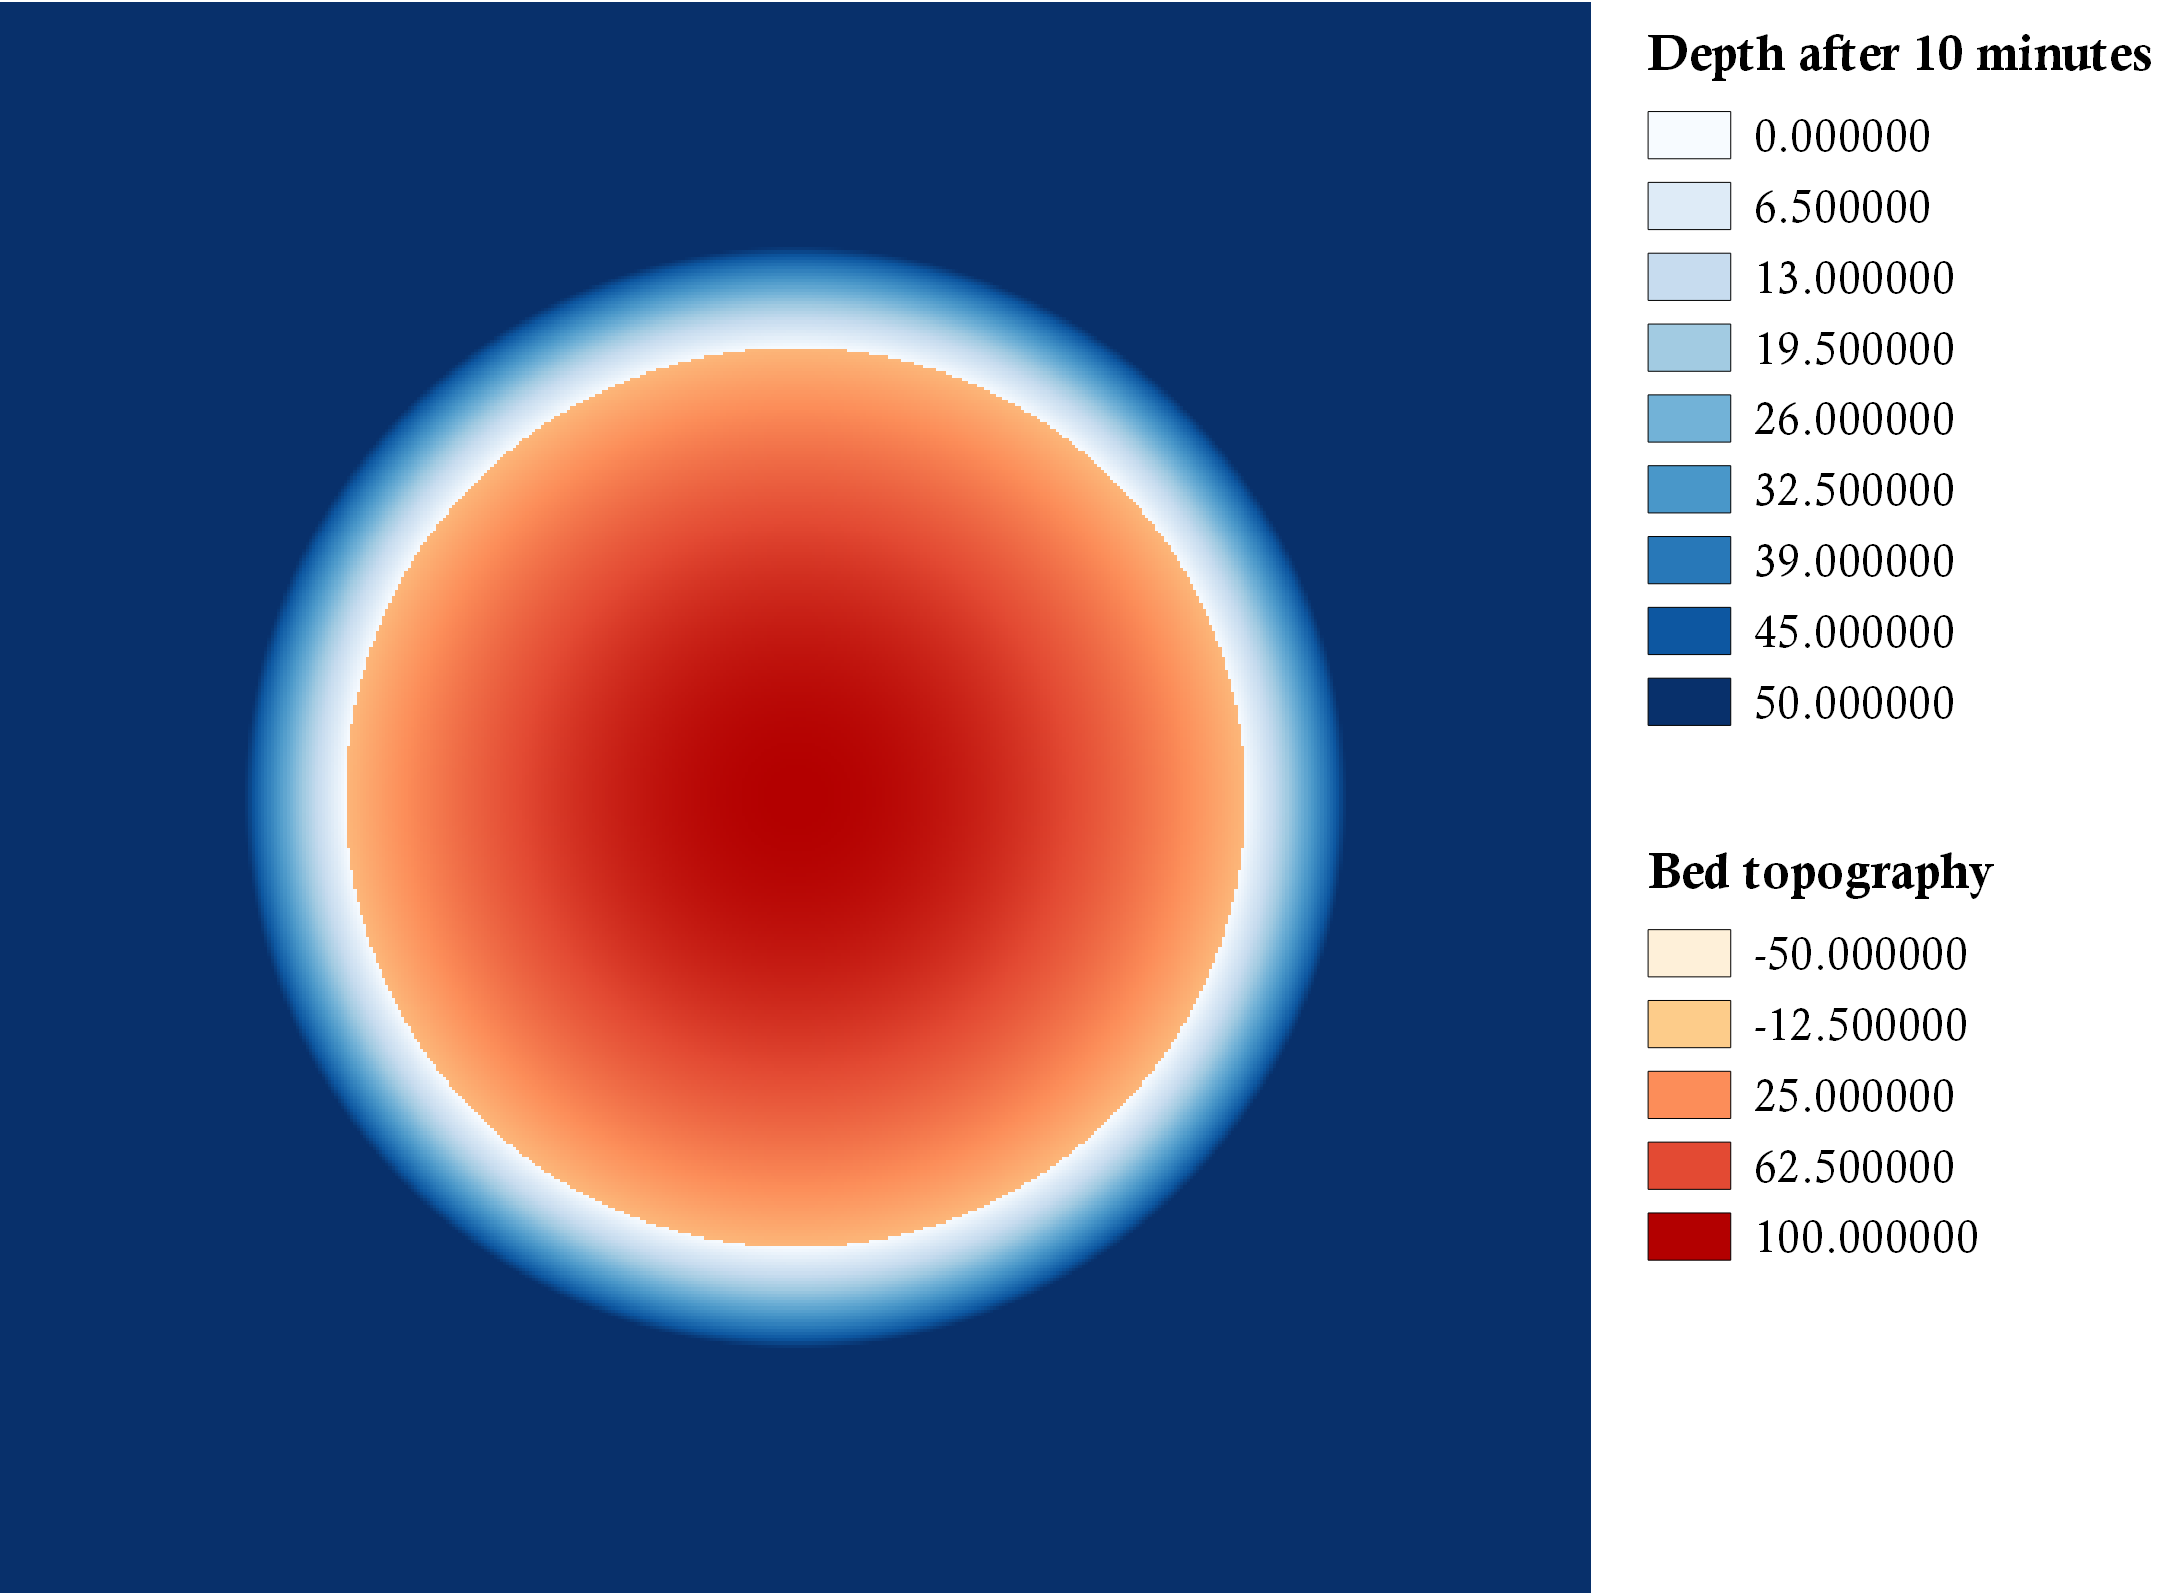
\includegraphics[width=0.9\textwidth]{numerical-test-figures/well-balanced-10mins.png}
	\caption{Depth within the domain after a 10 minute period, with the high points of the topography seen dry in the centre.}
	\label{TestResult_WellBalanced}
\end{figure*}

\section{Moving wet-dry fronts}

\begin{figure*}[tpb]
	\centering
	\begin{tabular}{cc}
		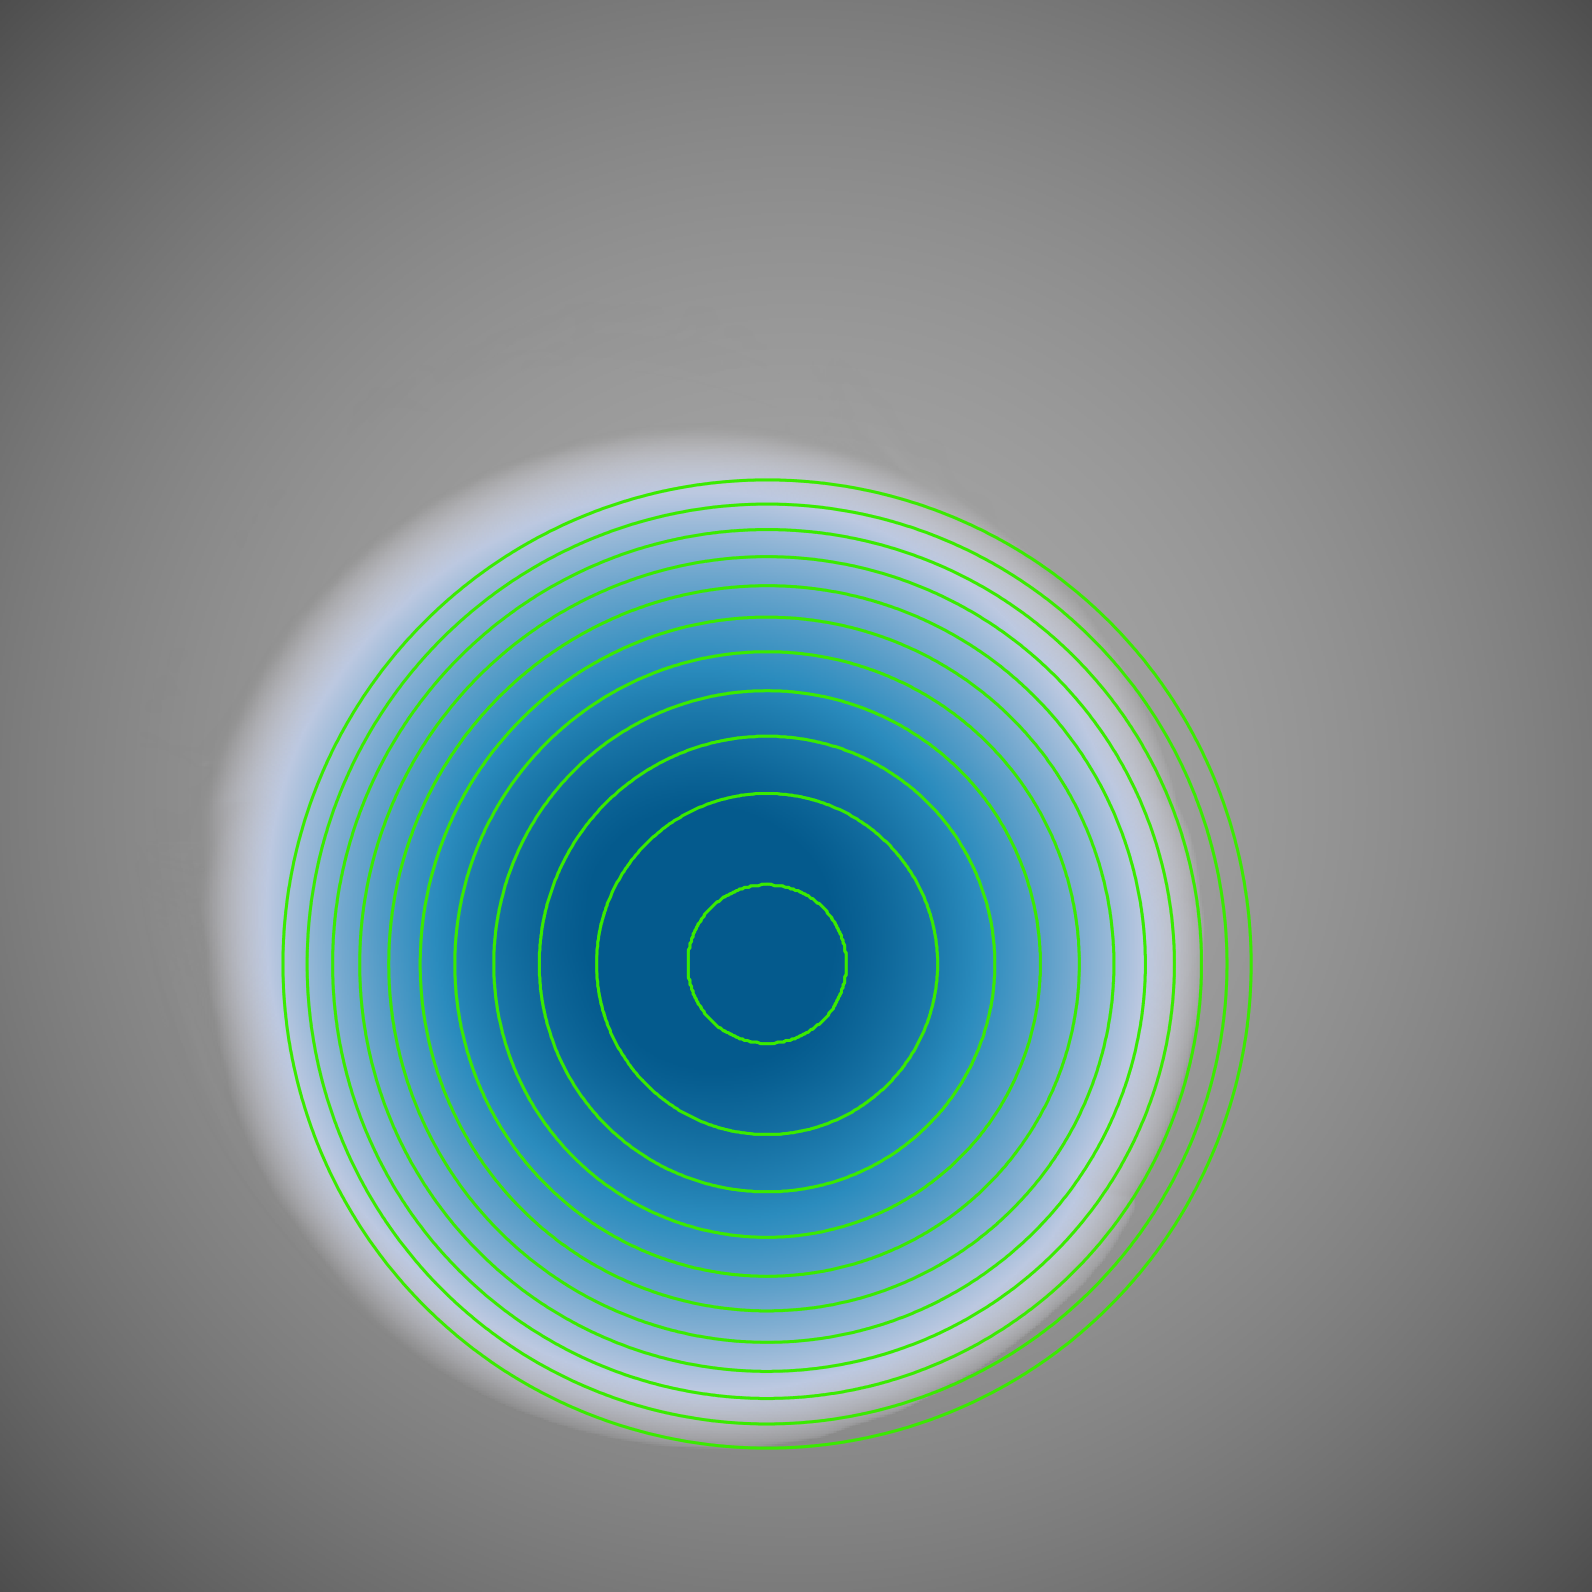
\includegraphics[width=0.4\textwidth]{numerical-test-figures/parabolic-bowl-1O-depth-300s.png} &
		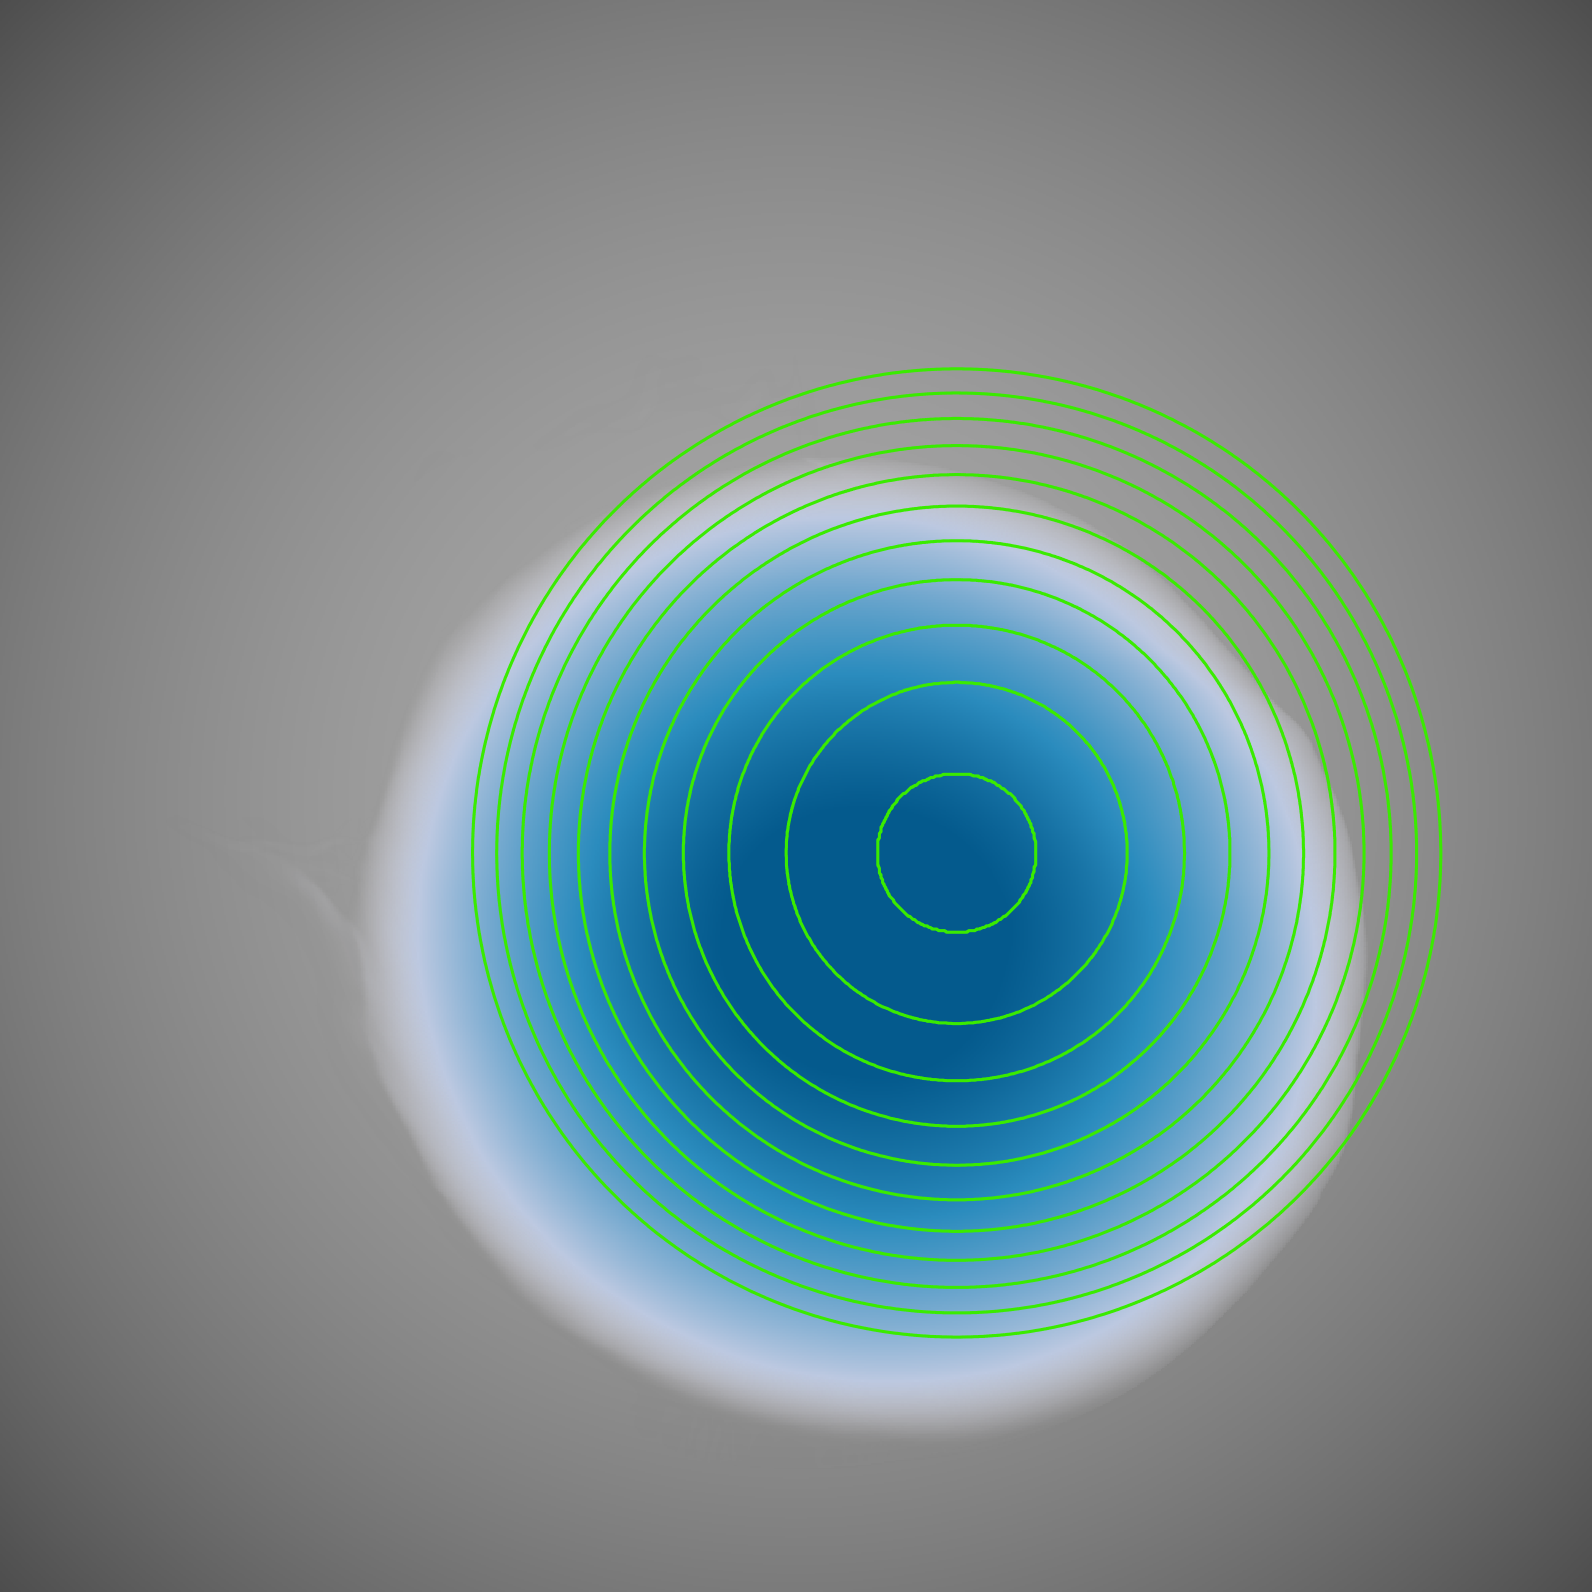
\includegraphics[width=0.4\textwidth]{numerical-test-figures/parabolic-bowl-1O-depth-600s.png} \\
		(a) 300s &
		(b) 600s \\[6pt]
		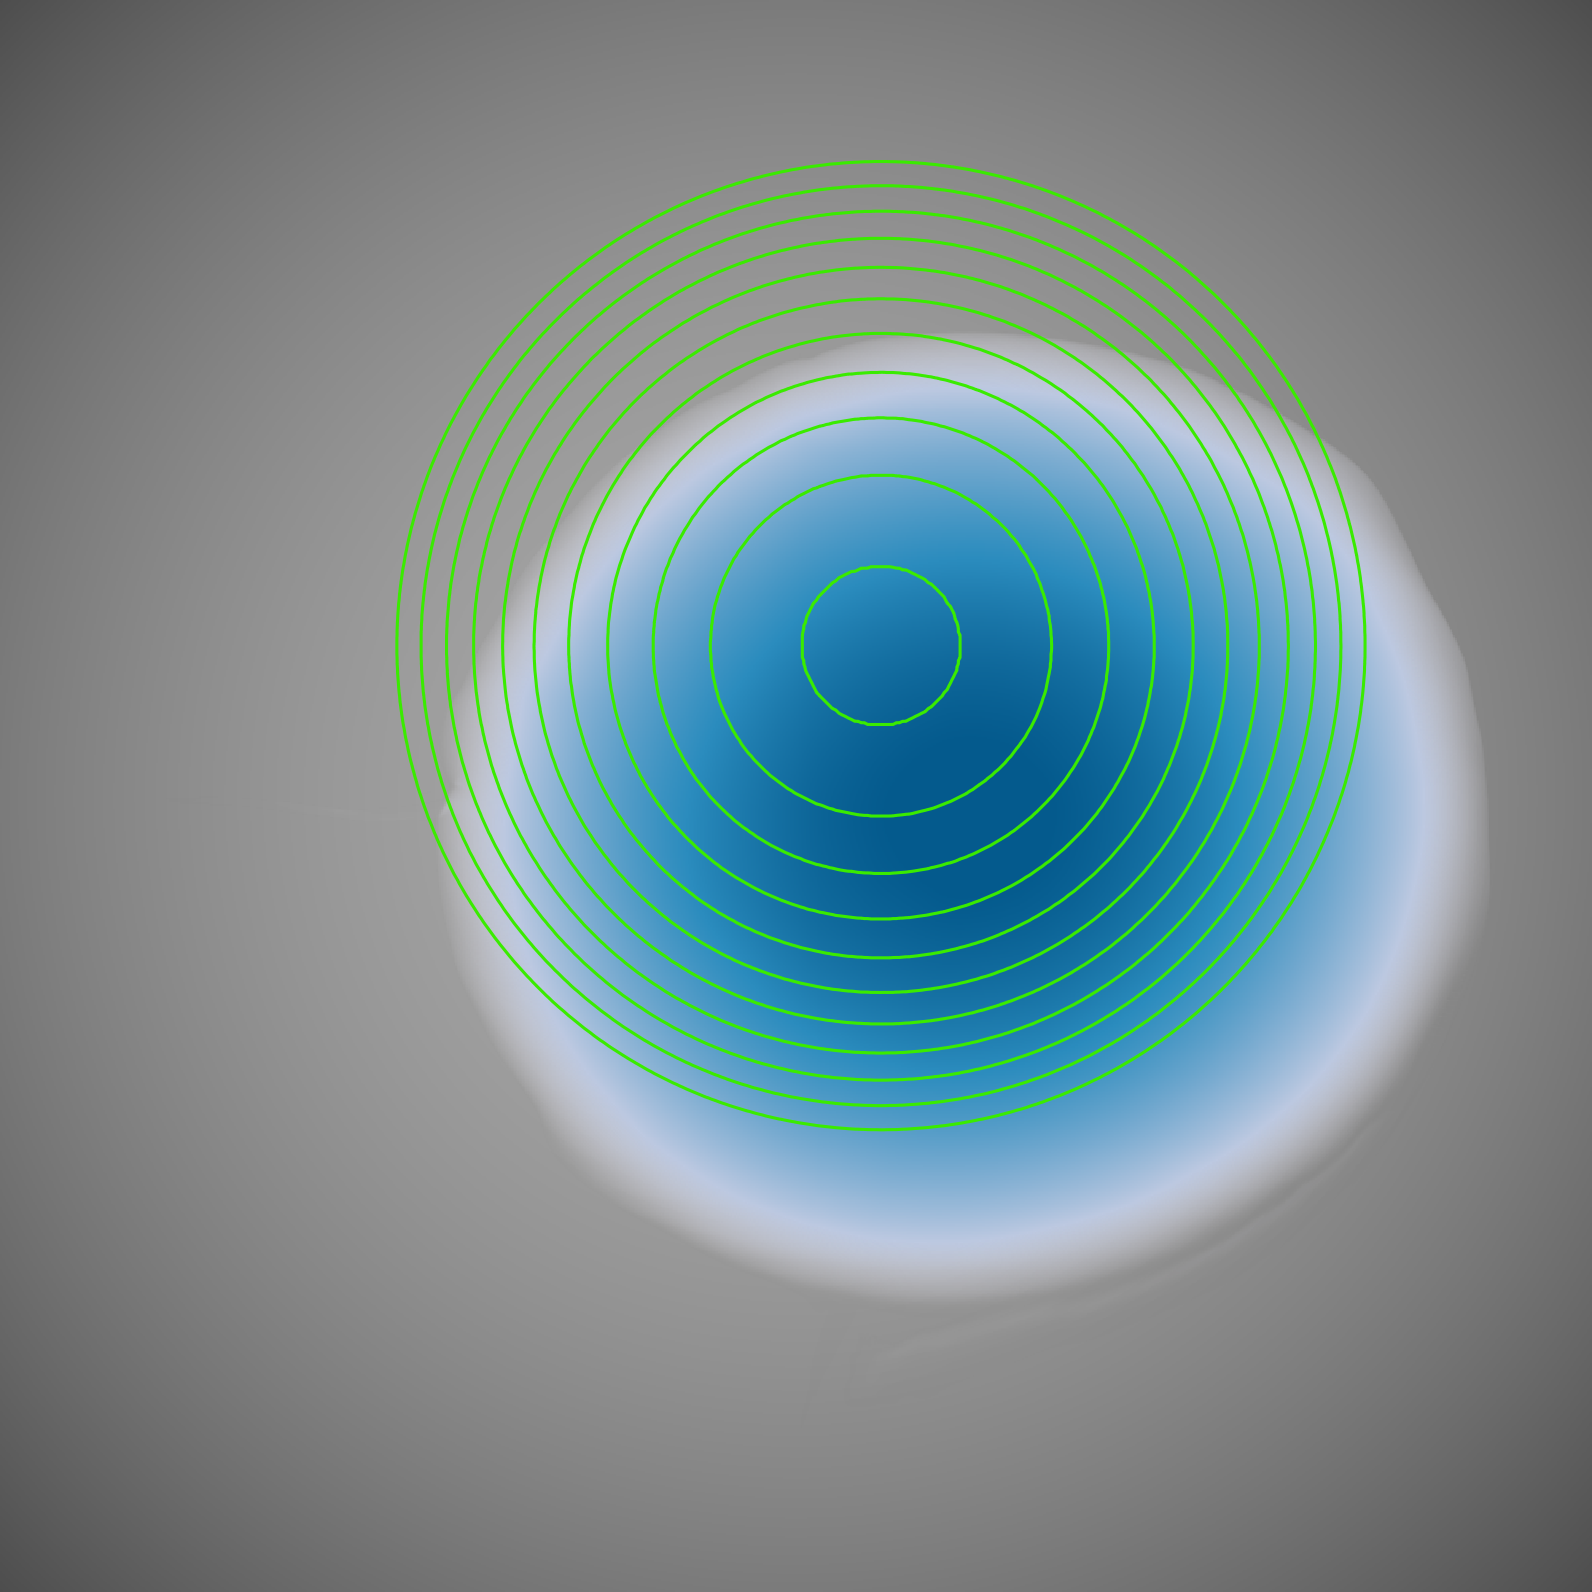
\includegraphics[width=0.4\textwidth]{numerical-test-figures/parabolic-bowl-1O-depth-900s.png} &
		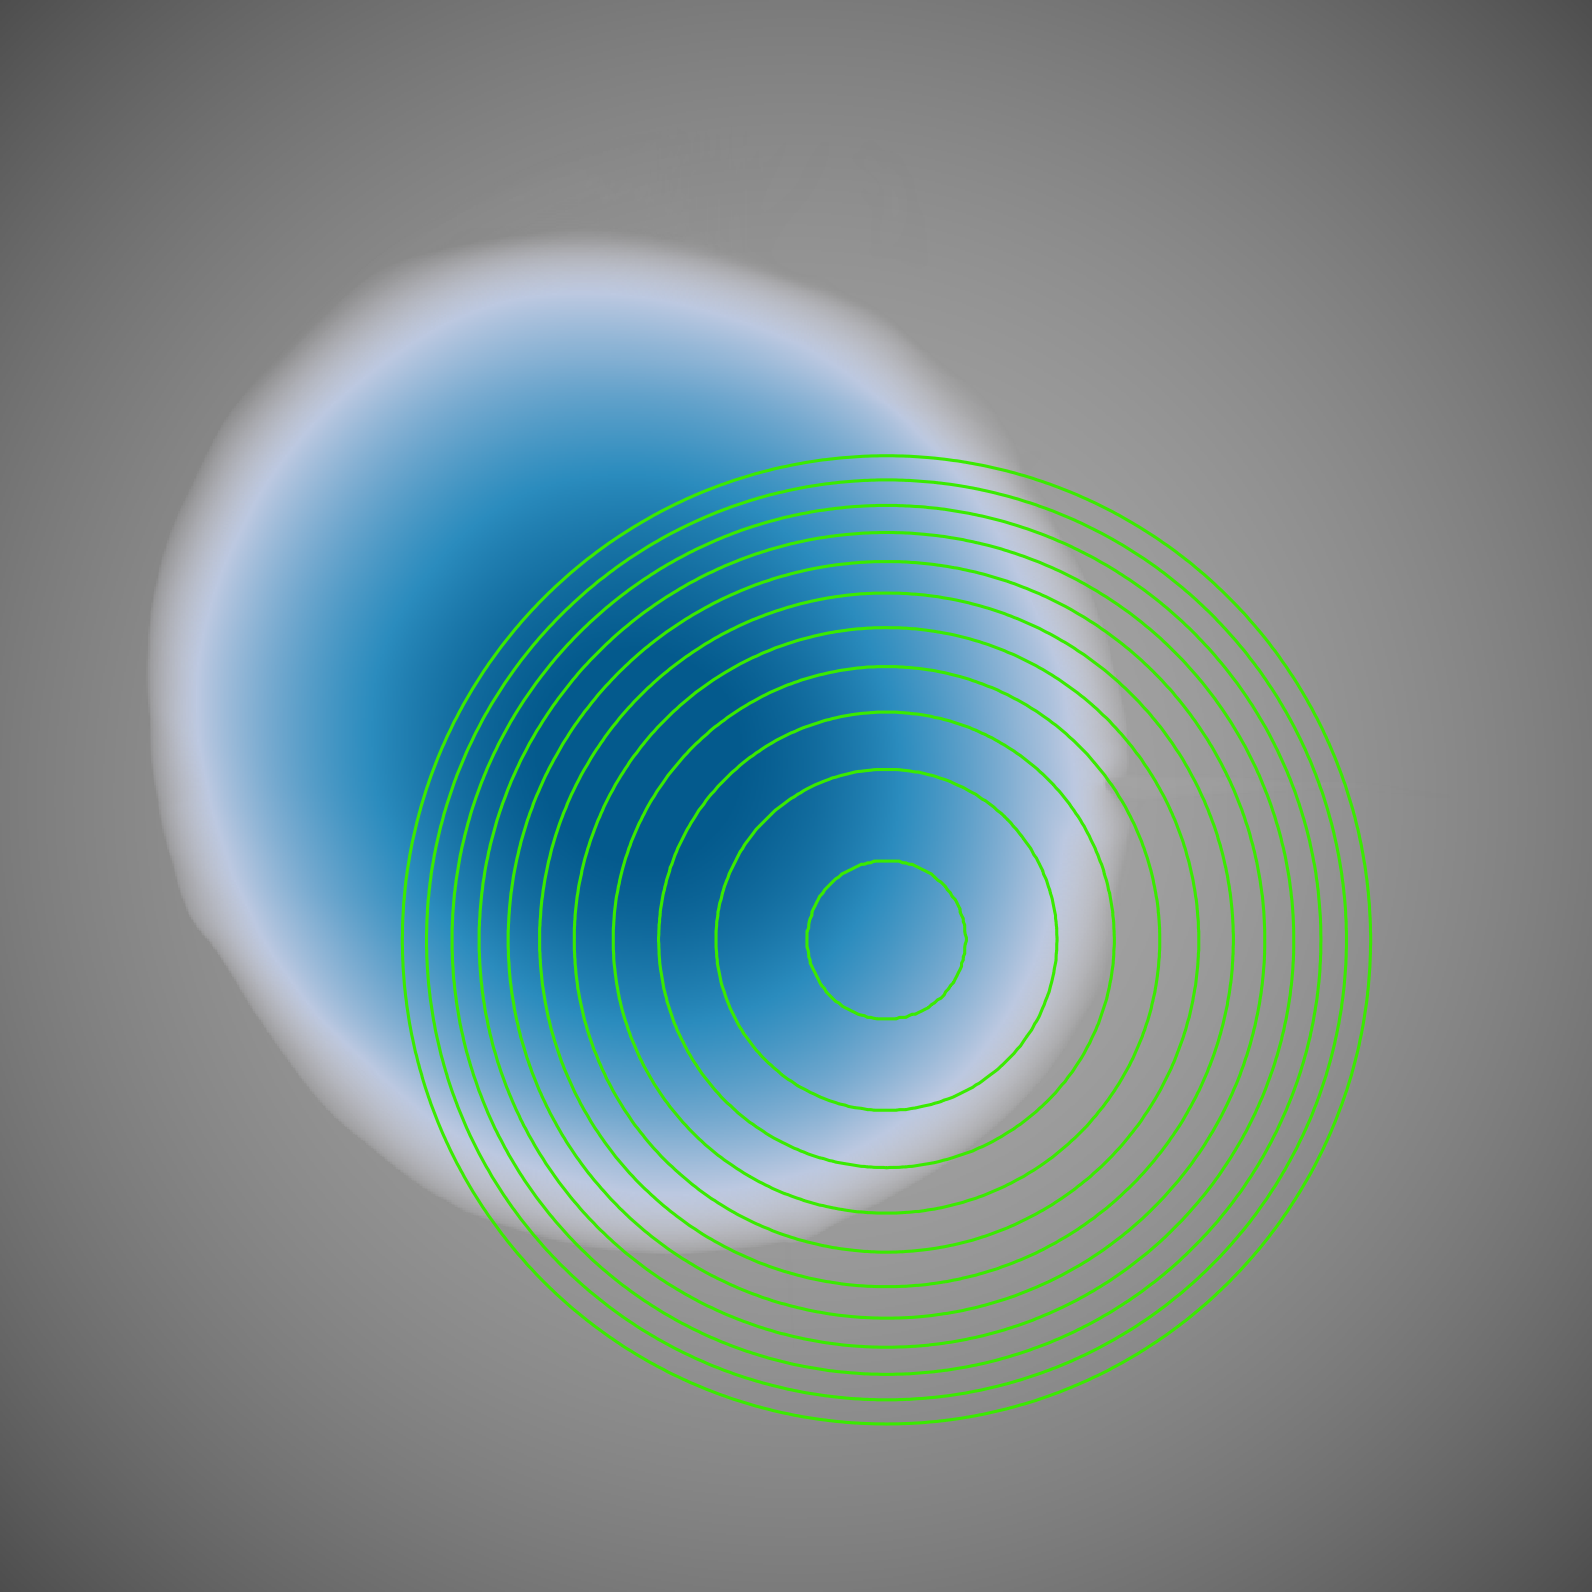
\includegraphics[width=0.4\textwidth]{numerical-test-figures/parabolic-bowl-1O-depth-1800s.png} \\
		(c) 900s &
		(d) 1800s \\[6pt]
		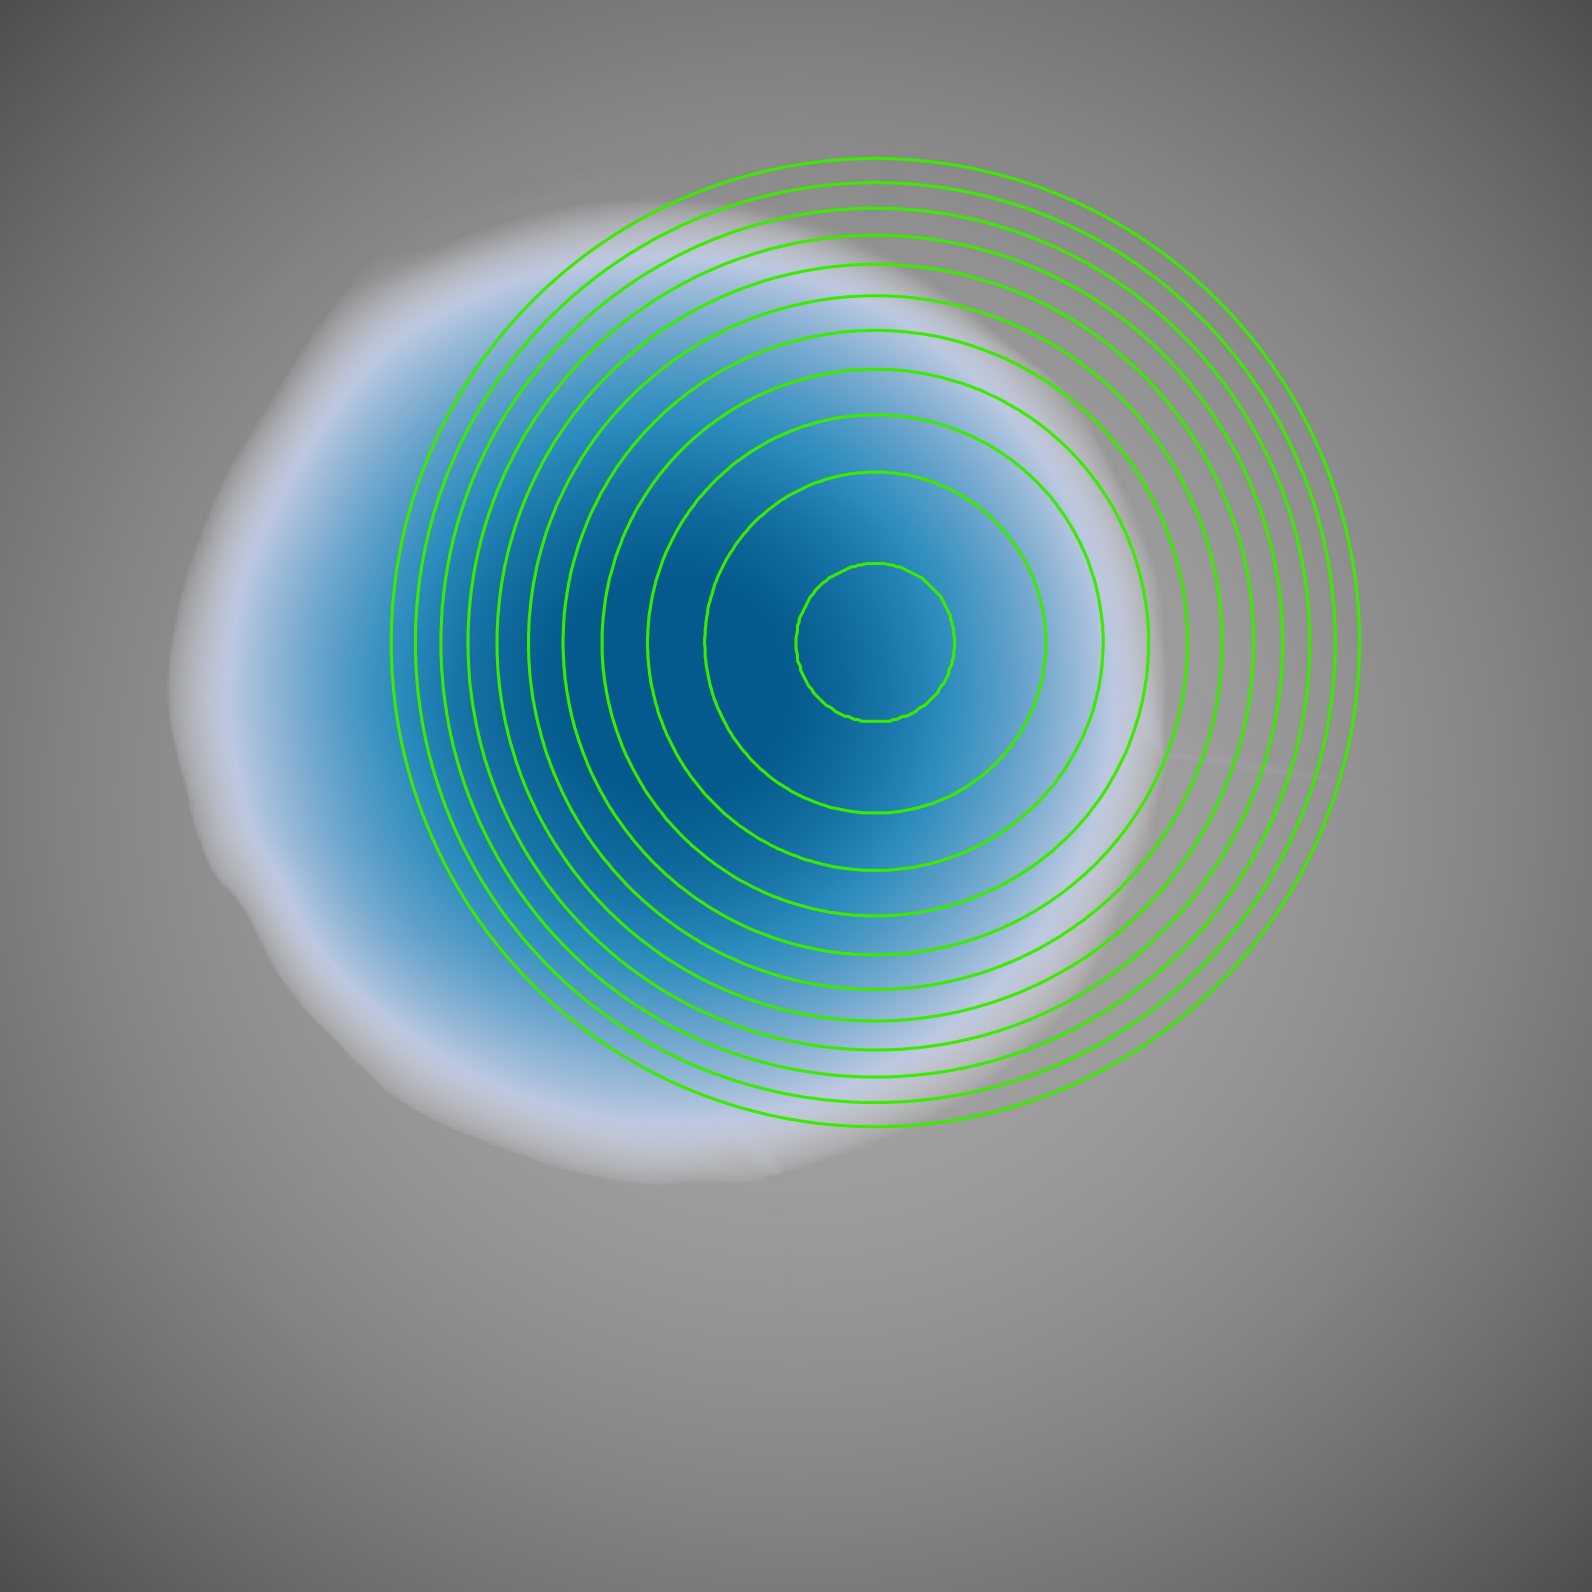
\includegraphics[width=0.4\textwidth]{numerical-test-figures/parabolic-bowl-1O-depth-3600s.png} &
		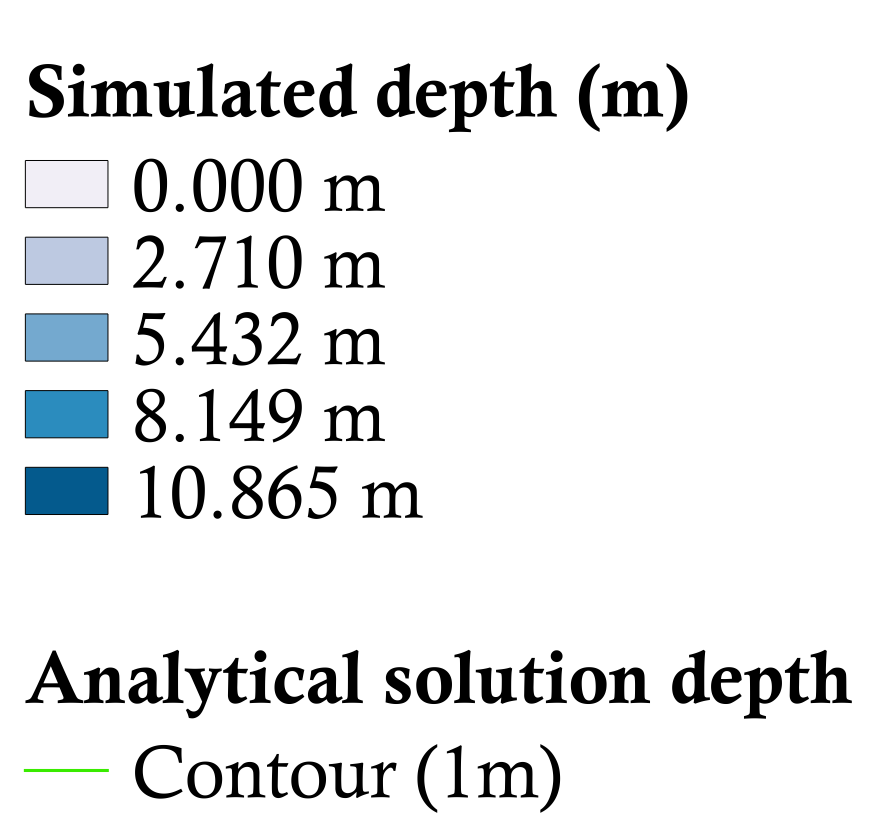
\includegraphics[width=0.26\textwidth]{numerical-test-figures/parabolic-bowl-depth-legend.png} \\
		(e) 3600s &
	\end{tabular}
	\caption{Comparison between analytical solution depth (contours) and simulation results, for first-order solutions.}
	\label{TestResult_ParabolicBowl_1O}
\end{figure*}
\begin{figure*}[tpb]
	\centering
	\begin{tabular}{cc}
		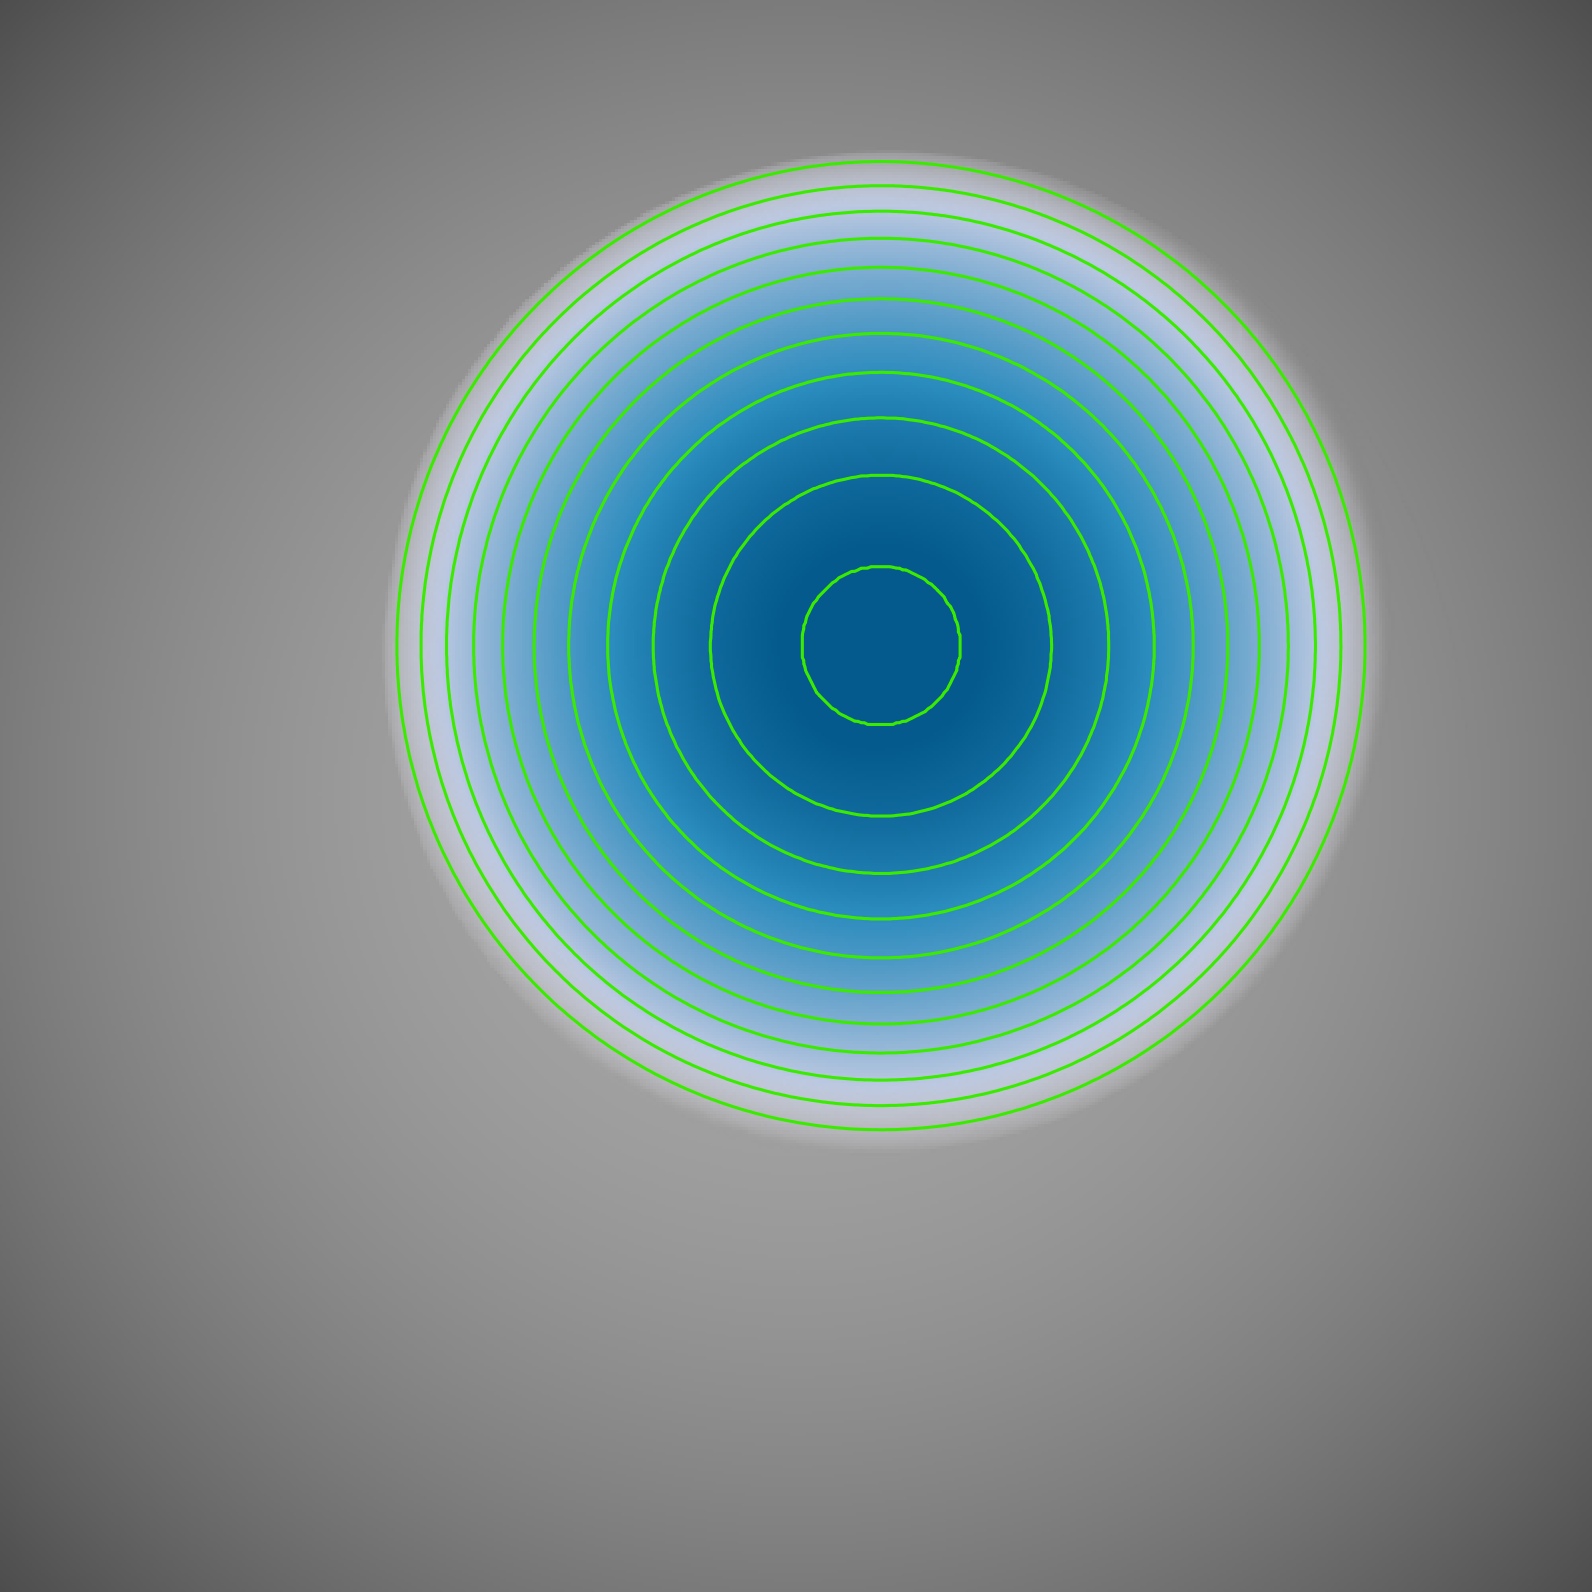
\includegraphics[width=0.4\textwidth]{numerical-test-figures/parabolic-bowl-2O-depth-900s.png} &
		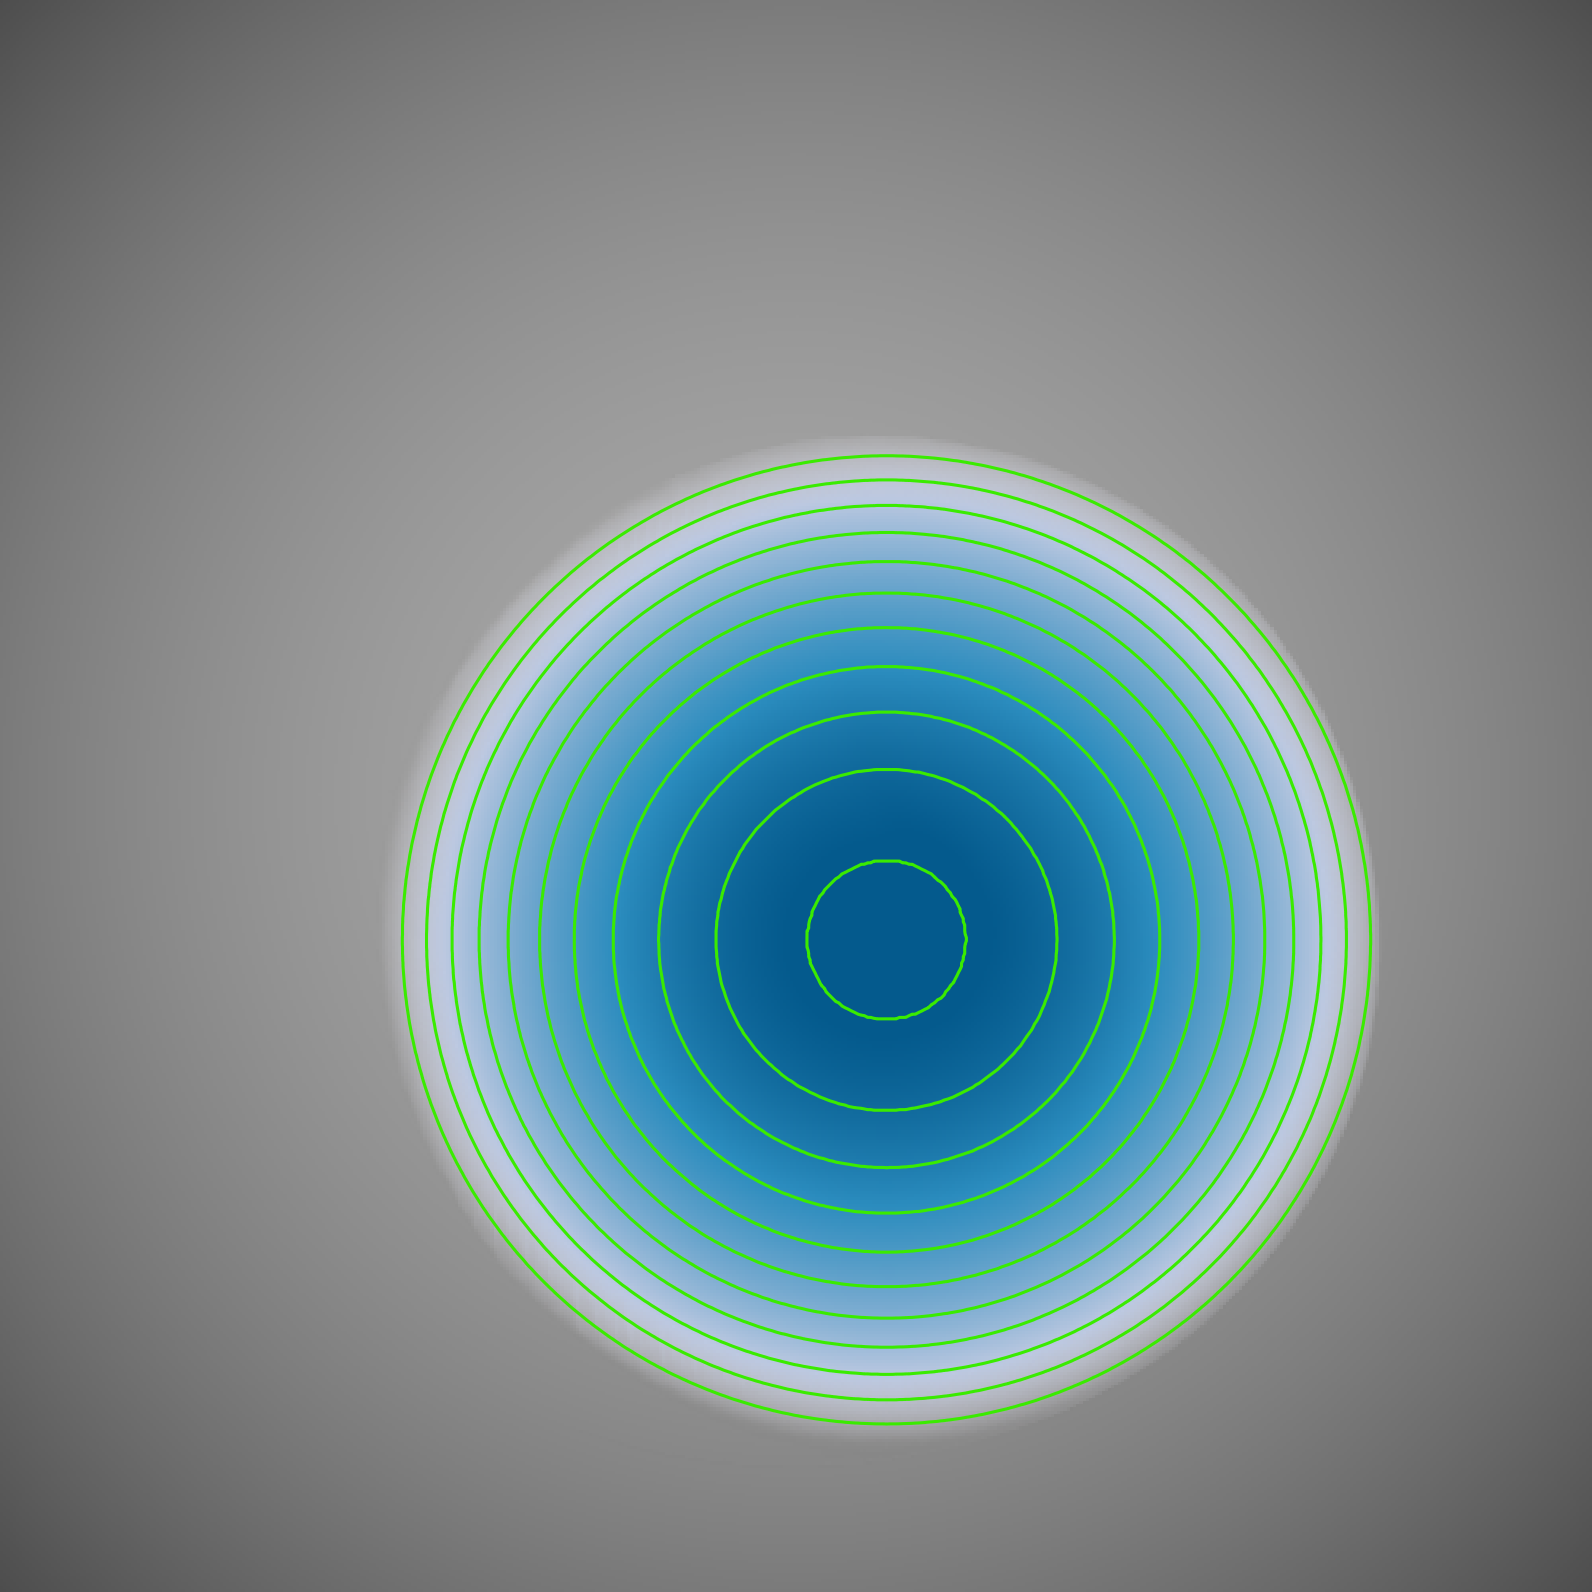
\includegraphics[width=0.4\textwidth]{numerical-test-figures/parabolic-bowl-2O-depth-1800s.png} \\
		(a) 900s &
		(b) 1800s \\[6pt]
		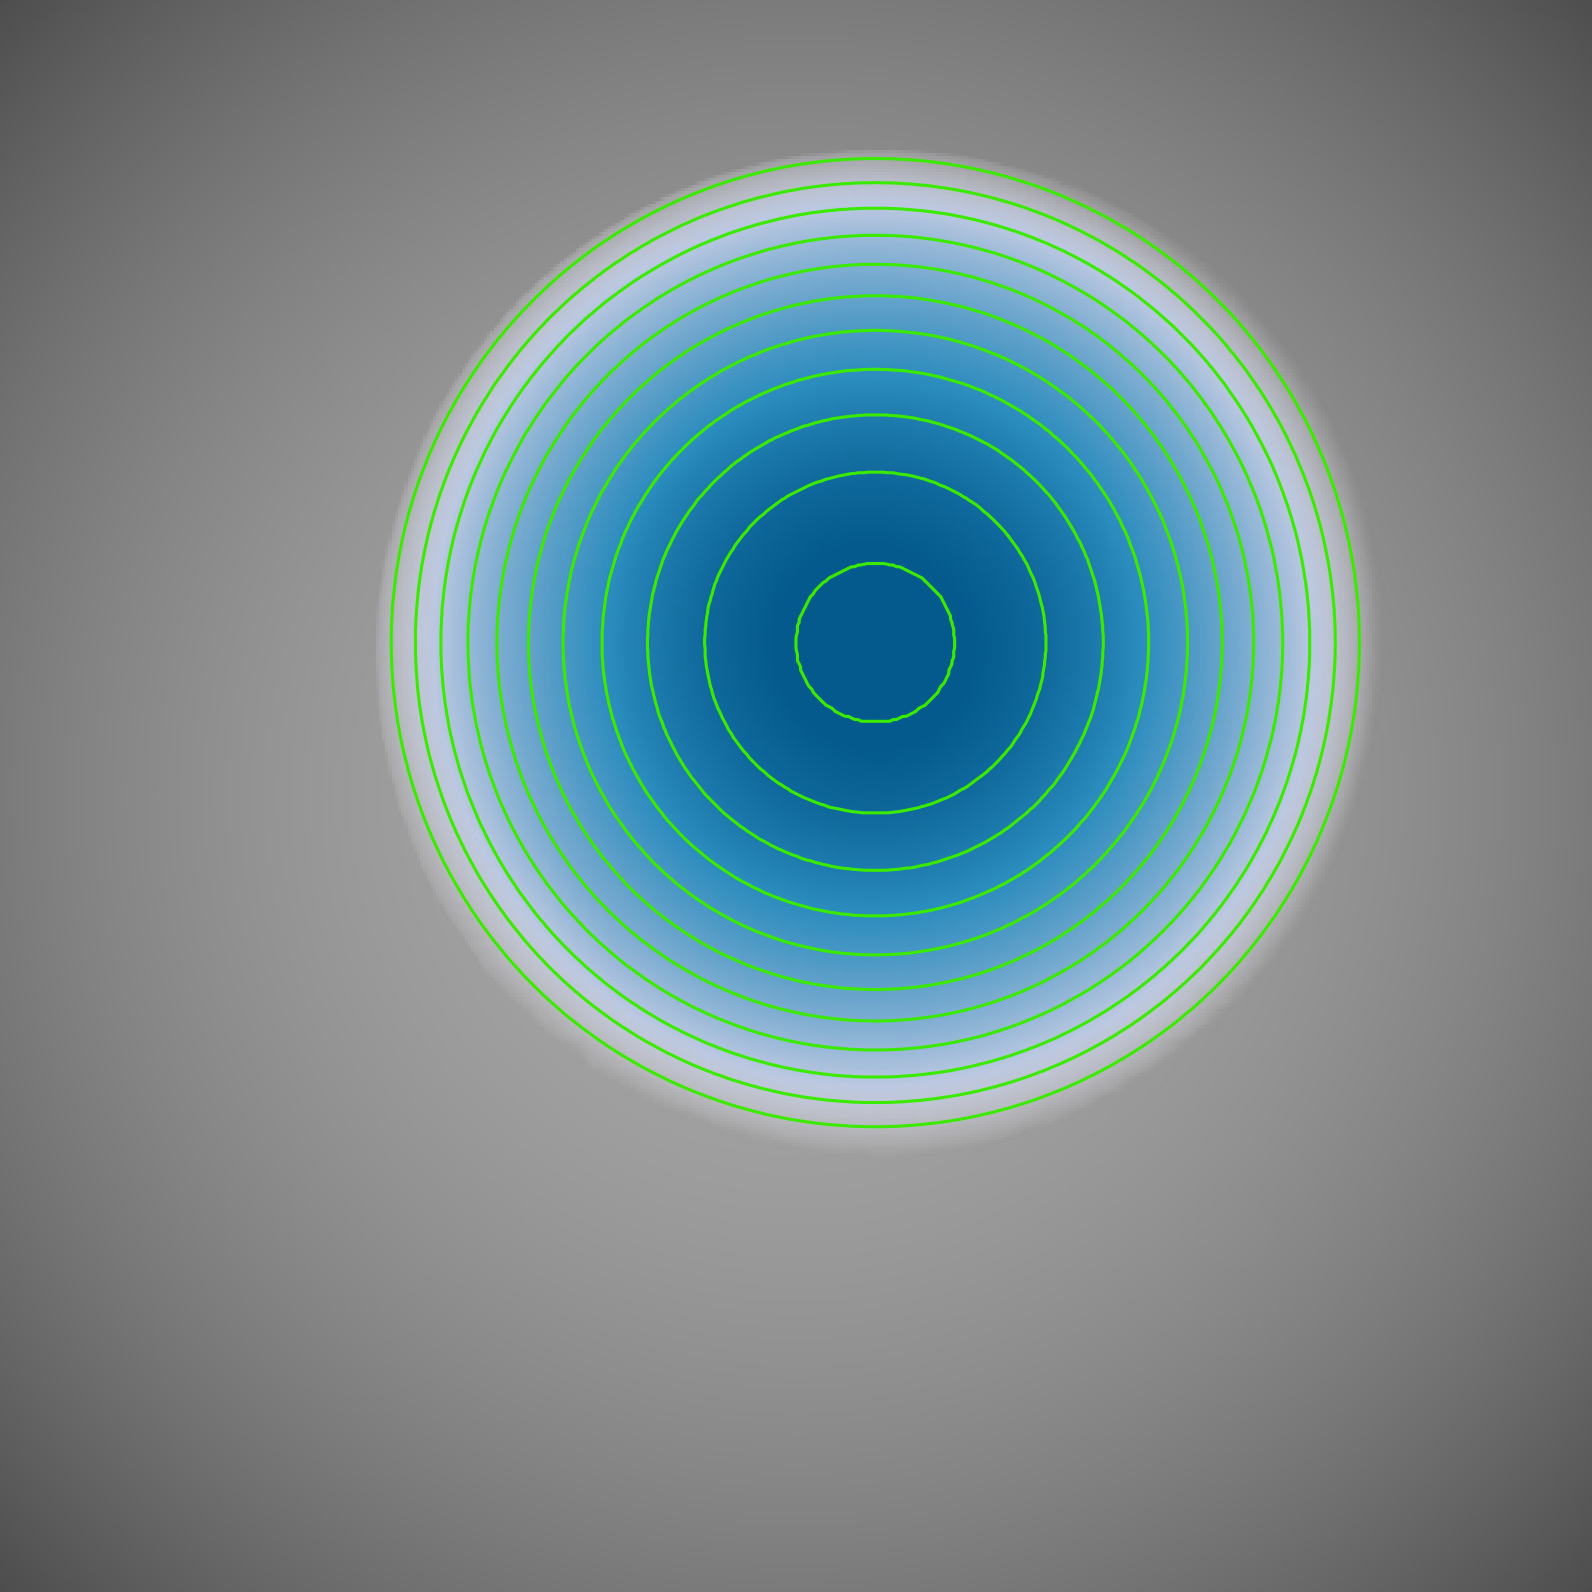
\includegraphics[width=0.4\textwidth]{numerical-test-figures/parabolic-bowl-2O-depth-3600s.png} &
		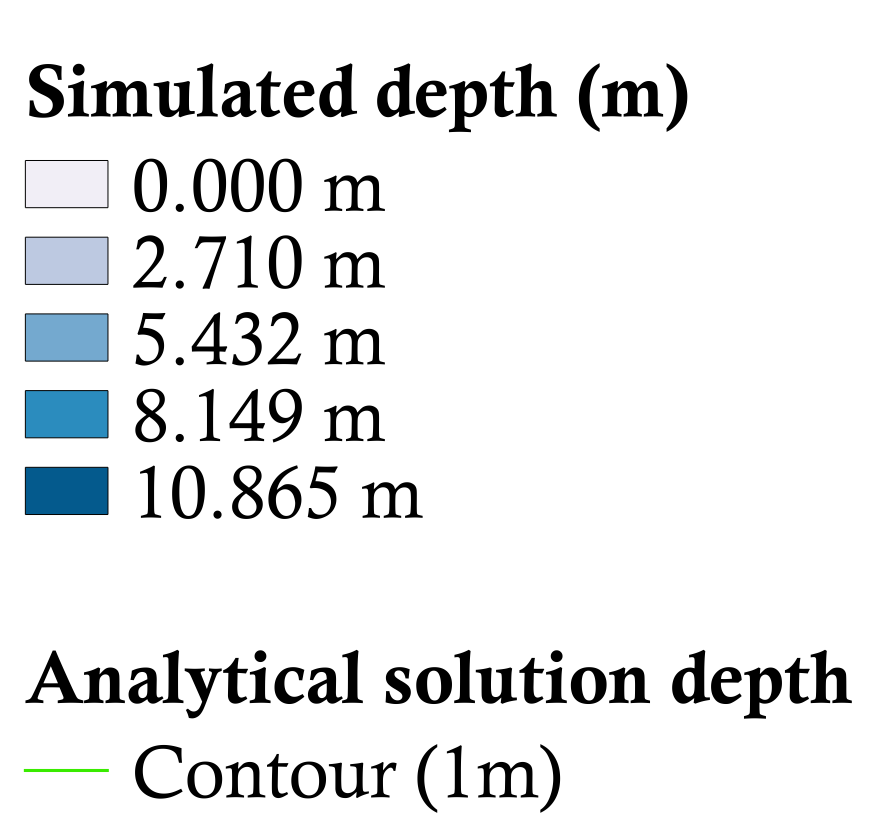
\includegraphics[width=0.26\textwidth]{numerical-test-figures/parabolic-bowl-depth-legend.png} \\
		(c) 3600s &
	\end{tabular}
	\caption{Comparison between analytical solution depth (contours) and simulation results, for second-order solutions.}
	\label{TestResult_ParabolicBowl_2O}
\end{figure*}

Constantly changing wet and dry fronts provide a more challenging situation for the numerical scheme, but are representative of situations arising during pluvial, fluvial, and tidal flooding situations. An analytical solution is known for the case of a parabolic bowl, with water travelling at a velocity around the bowl, and friction neglected such that there is no reduction in velocity with time. A correct solution should theoretically forecast the position of the wet-dry fronts at any point in time, while numerical diffusion is expected to manifest as a gradually increasing deformity in the shape of the flow. Derivation and more comprehensive details for the test case are provided in \citet{Wang2011}.

A scaling factor $h_0 = 10.0$, sloping factor $\alpha = 3000.0$, initial velocity $\beta = 5.0$ and friction parameter of $\tau = 0.0$ are used herein, with the derivative constants,
\begin{equation}
\label{Test_ParabolicBowl_Derivatives}
a = \sqrt{8 g \frac{h_0}{\alpha^2}}, \\
S = \frac{\sqrt{a^2 - \tau^2}}{2}
.
\end{equation}

The initial conditions and analytical results are thus described,
\begin{equation}
\label{Test_ParabolicBowl_Conditions}
\begin{alignedat}{2}
z_b & = h_0 \frac{x^2 + y^2}{\alpha^2}, \\
\eta & = h_0 - \frac{1}{g} \beta e^{\displaystyle-\frac{\tau t}{2}} \times \left( \frac{\tau}{2} sin(St) + S cos(St) \right) x \\
& - \frac{1}{g} \beta e^{\displaystyle-\frac{\tau t}{2}} \times \left( \frac{\tau}{2} cos(St) + S sin(St) \right) y, \\
u & = \beta e^{\displaystyle-\frac{\tau t}{2}} sin(St), \\
v & = -\beta e^{\displaystyle-\frac{\tau t}{2}} cos(St),
\end{alignedat}
\end{equation}
where $t = 0.0$ for initial conditions.

Results for the first-order case at different time periods are presented in Figure \ref{TestResult_ParabolicBowl_1O}. A correct solution has the analytical result overlapping the simulation, whereas it is clearly visible that the error grows as time passes. This is a consequence of numerical dispersion. The overall behaviour however is nonetheless represented correctly. 

A similar figure is provided for the results of a second-order MUSCL-Hancock simulation in Figure \ref{TestResult_ParabolicBowl_2O}, where despite the numerical scheme's requirement to fall back to first-order solutions along wet-dry fronts, to the advantage of numerical stability, the overall simulation result matches almost exactly with the analytical solution.

\section{Dam-break simulation over an emerging bed}

The results provided so far in this chapter, have not sufficiently tested the numerical scheme's capability for capturing the behaviour of shocks, encompassing hydraulic jump phenomena, and other such complexities encountered in the real world. The failure of a dam, in which water rapidly leaves a body of water with considerable depth, creates high velocities and may result in a hydraulic jump. A theoretical dam break over an emerging bed is therefore considered, whereby the inclined bed removes energy from the oncoming wave. A wall is provided around the extremity of the domain, such as to contain the flow, and with a thickness of two cells thereby ensuring all cells which will become inundated are included in the computational domain, with respect to the earlier discussions on cell data requirements in first- and second-order solutions. This is an adaptation of the example employed by \citet{Xing2010}.

Only the MUSCL-Hancock scheme is employed, as the most appropriate scheme for the flow under consideration. No friction effects are considered.

The initial conditions and domain are described as,
\begin{equation}
\label{Test_EmergingBed_Conditions}
\begin{alignedat}{4}
z_b & = x \cdot tan(\theta) &&, \\
u & = 0.0, && \\
v & = 0.0, && \\
d & = \eta && where \hspace{1cm} x < p,
\end{alignedat}
\end{equation}
where constants are $\displaystyle\theta = \frac{\pi}{60}, \eta = 1.0, p = 0.0$. The domain is considered to be 30.00m in length, 0.35m in width, and represented by 4,200 cells of resolution 0.05m, with the grid origin in the centre of the domain. This provides sufficient room for the shock and rarefaction waves to propagate without encountering the extremity of the domain for the first few seconds.

\begin{sidewaysfigure}
	\centering
	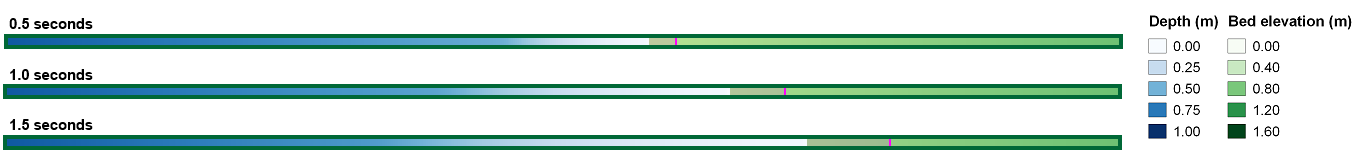
\includegraphics[width=1.05\textheight]{numerical-test-figures/dam-break-emerging-bed-example.png}
	\caption{Comparison between the inundated area in simulation results, and the analytical solution for the position of the front (shown as a line), for the dam-break against an emerging bed test.}
	\label{TestResult_EmergingBed}
\end{sidewaysfigure}

The position of the front is determined by,
\begin{equation}
\label{Test_EmergingBed_FrontPosition}
x_{front} = 2t \sqrt{g h_0 cos(\theta)} - \frac{gt^2 \cdot tan(\theta)}{2},
\end{equation} and shown against the simulation results in Figure \ref{TestResult_EmergingBed}.

The limitations of the numerical methods and modelling employed are clear in the results, with the simulated front progressively further from the analytically-derived front. In this case, especially against the adverse gradient of the domain, it is possible that the second-order method falling back to first-order at the wet-dry front is not sufficiently alleviating the numerical diffusion effects. Moreover, it is also worth considering, that the scheme employed is two-dimensional and relies upon depth-averaged velocities and shallow water assumptions, as discussed in the comparative study of \citet{Liang2010}. The author does not believe these results to be of particular concern, especially considering that the correct behaviour is exhibited by the simulation, and the likelihood that  limitations observed would likely require extension to three dimensions, and considerably more complex and expensive numerical methods, to achieve any significant improvement in the results. 

\section{Dam-break against a fixed obstacle}

\begin{sidewaysfigure}
	\centering
	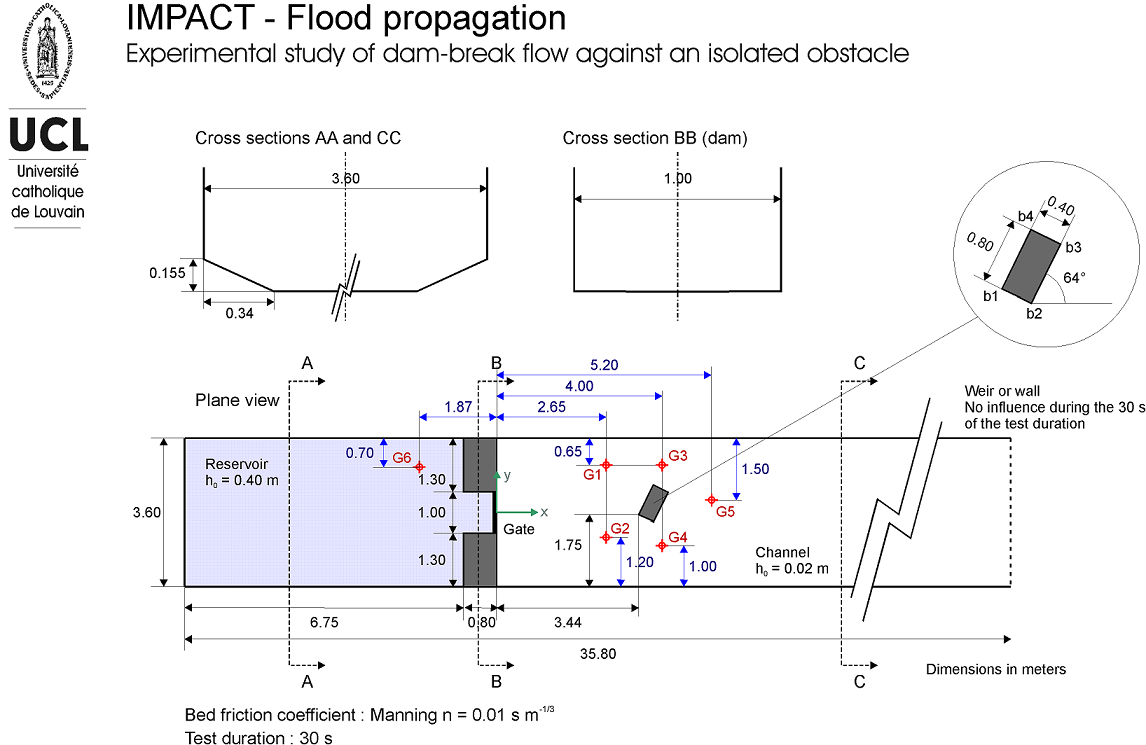
\includegraphics[width=1.0\textwidth]{numerical-test-figures/dam-break-obstacle-layout.png}
	\caption{Layout for the dam-break against an obstacle, showing the position of the gauges, position of the grid origin, and location of the obstacle.}
	\label{TestResult_DamObstacle_Domain}
\end{sidewaysfigure}

A dam-break against an obstacle presents a more complex situation again, for which there is no analytical solution. In practice, any dam failure would undoubtedly result in flow against obstacles, hence this is a useful test. A laboratory study conducted as part of the IMPACT project provides measurements and sufficient data to reproduce the situation in a simulation \citep{SoaresFrazao2007}. The dimensions of the domain and locations of gauges are shown in Figure \ref{TestResult_DamObstacle_Domain}, which is represented by a 0.02m grid, hence 322,200 cells in total.

The complex interaction between the shock and rarefaction waves, and those reflected from the obstacle are shown in the simulation results after three seconds (Figure \ref{TestResult_DamObstacle_Depth}), in a pattern and manner consistent with those described by \citet{SoaresFrazao2007}, clearly showing areas of supercritical flow.

A comparison between gauge measurements and simulation results is given in Figure \ref{TestResult_DamObstacle_Gauges}, where the simulation clearly exhibits the correct behaviour, even if the exact measurements show discrepancies. The arrival of wave-fronts appears delayed in comparison to the observations, and is often followed by exaggerated levels upon arrival. This is likely to be a consequence of the limitations of the shallow water equations during the initial dam-break, which may be underestimating the initial velocity of the wave-front.

\begin{sidewaysfigure}
	\centering
	\begin{subfigure}{1.0\textheight}
	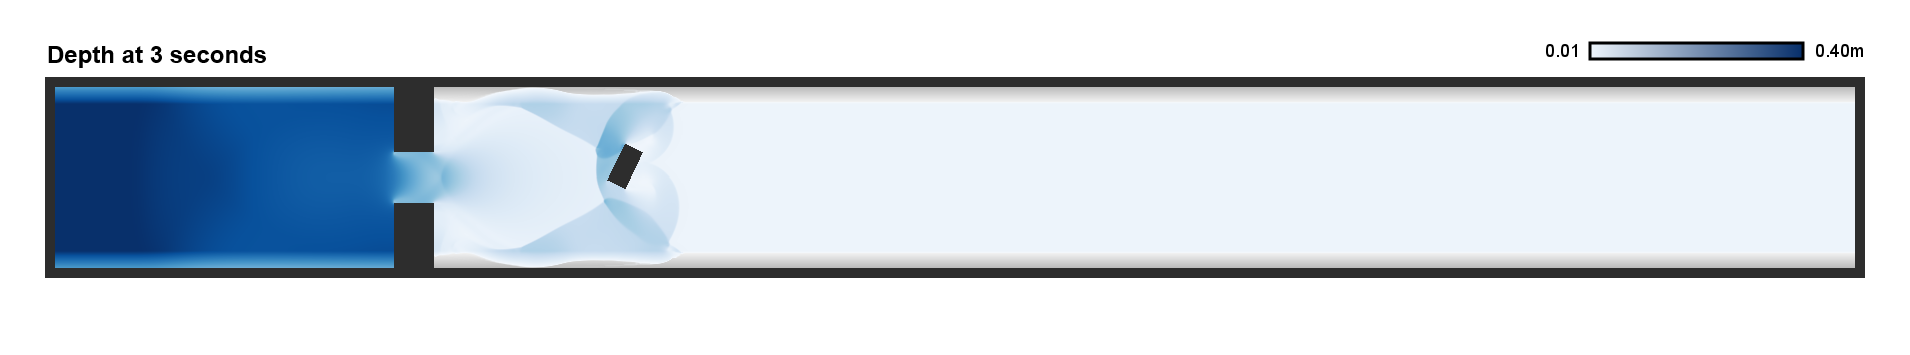
\includegraphics[width=1.0\textheight]{numerical-test-figures/dam-break-obstacle-depth-example.png}
	\caption{Depth, where darker colours are deeper, after a three second period.}
	\label{TestResult_DamObstacle_Depth}
	\end{subfigure}
	\begin{subfigure}{1.0\textheight}
	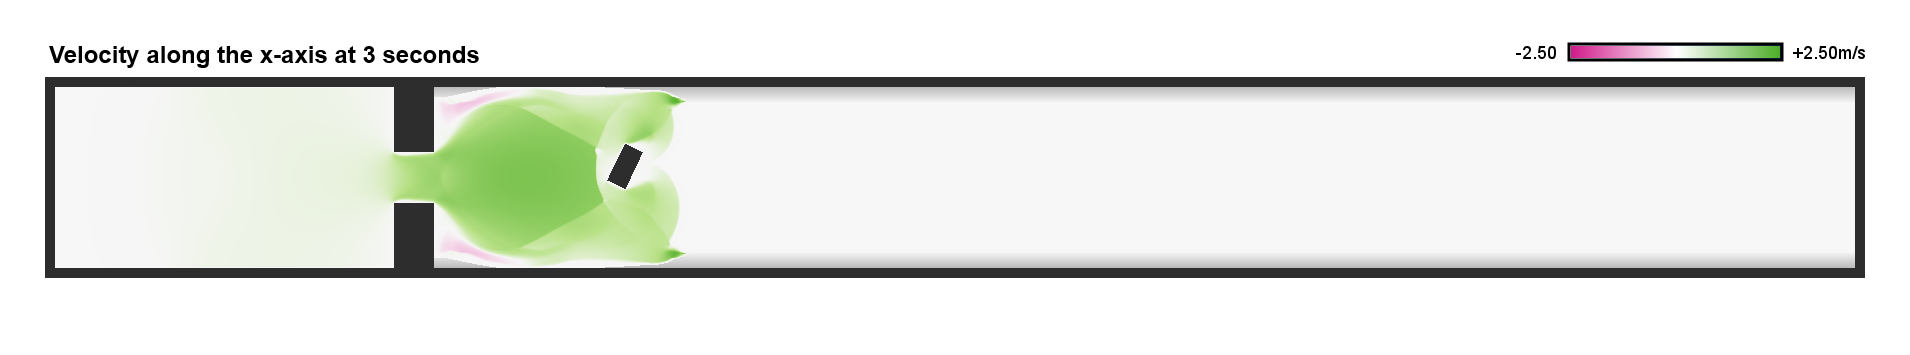
\includegraphics[width=1.0\textheight]{numerical-test-figures/dam-break-obstacle-velocity-example.png}
	\caption{Velocity, along $x$-axis where darker colours are higher, after a three second period.}
	\label{TestResult_DamObstacle_Velocity}
	\end{subfigure}
	\caption{Representation of depth and velocity in the dam break against an obstacle.}
\end{sidewaysfigure}
\begin{figure*}[tpb]
	\centering
	\begin{tabular}{cc}
		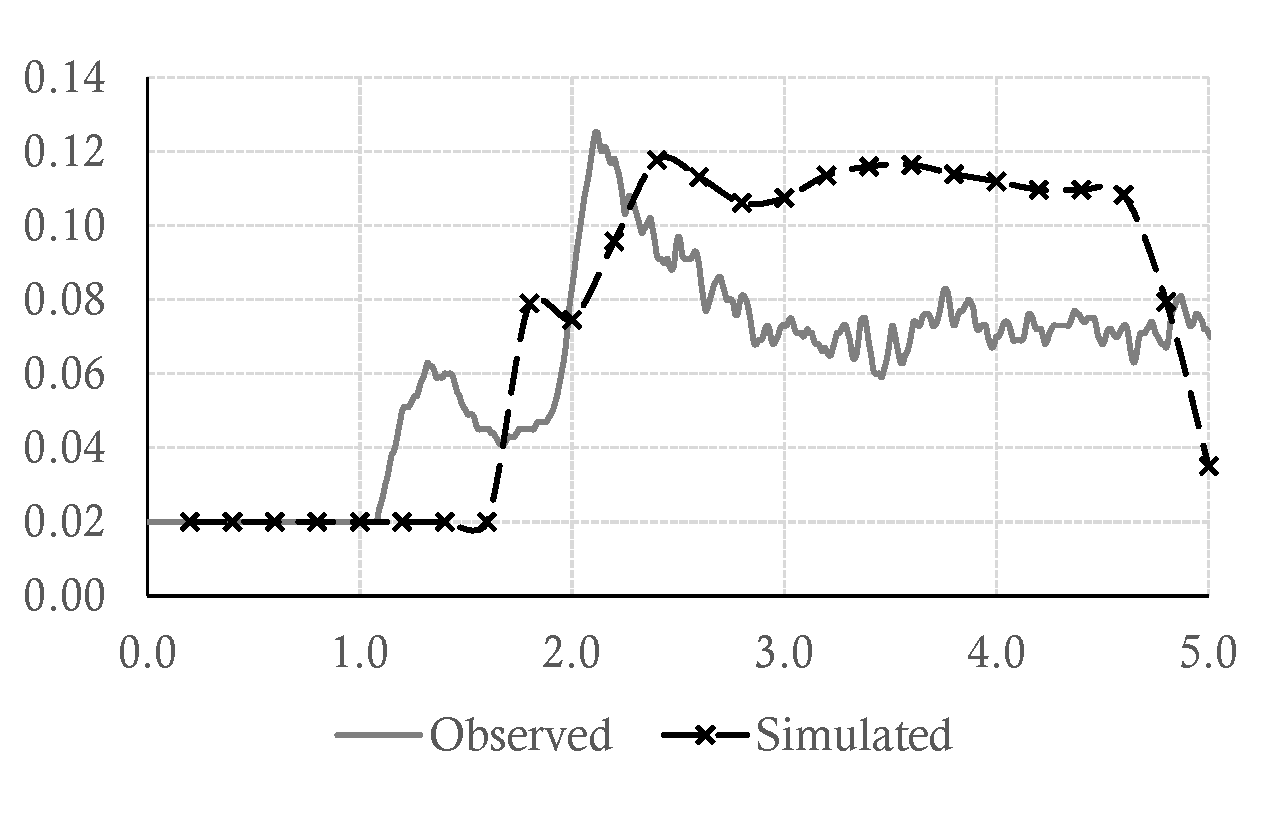
\includegraphics[width=0.5\textwidth]{numerical-test-figures/dam-break-obstacle-results-g1.pdf} &
		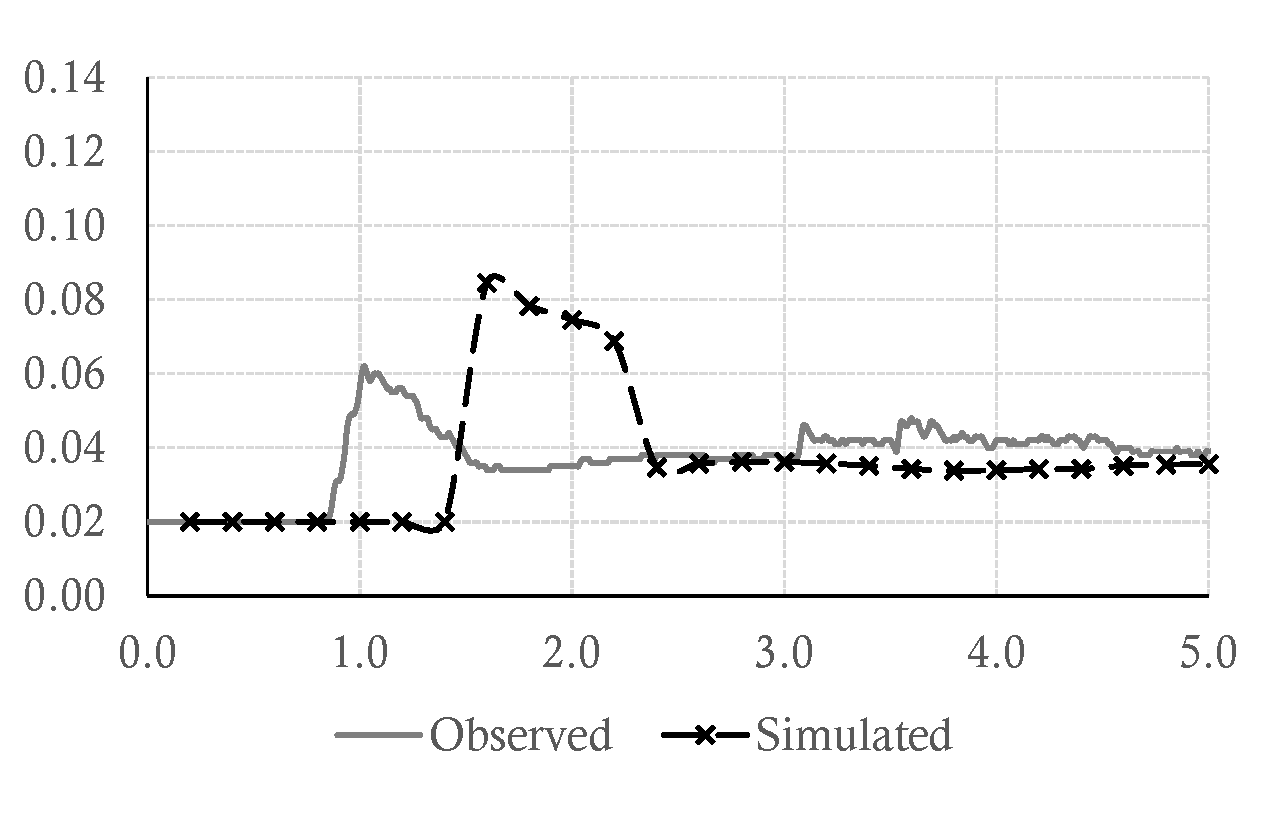
\includegraphics[width=0.5\textwidth]{numerical-test-figures/dam-break-obstacle-results-g2.pdf} \\
		(a) G1 &
		(b) G2 \\[6pt]
		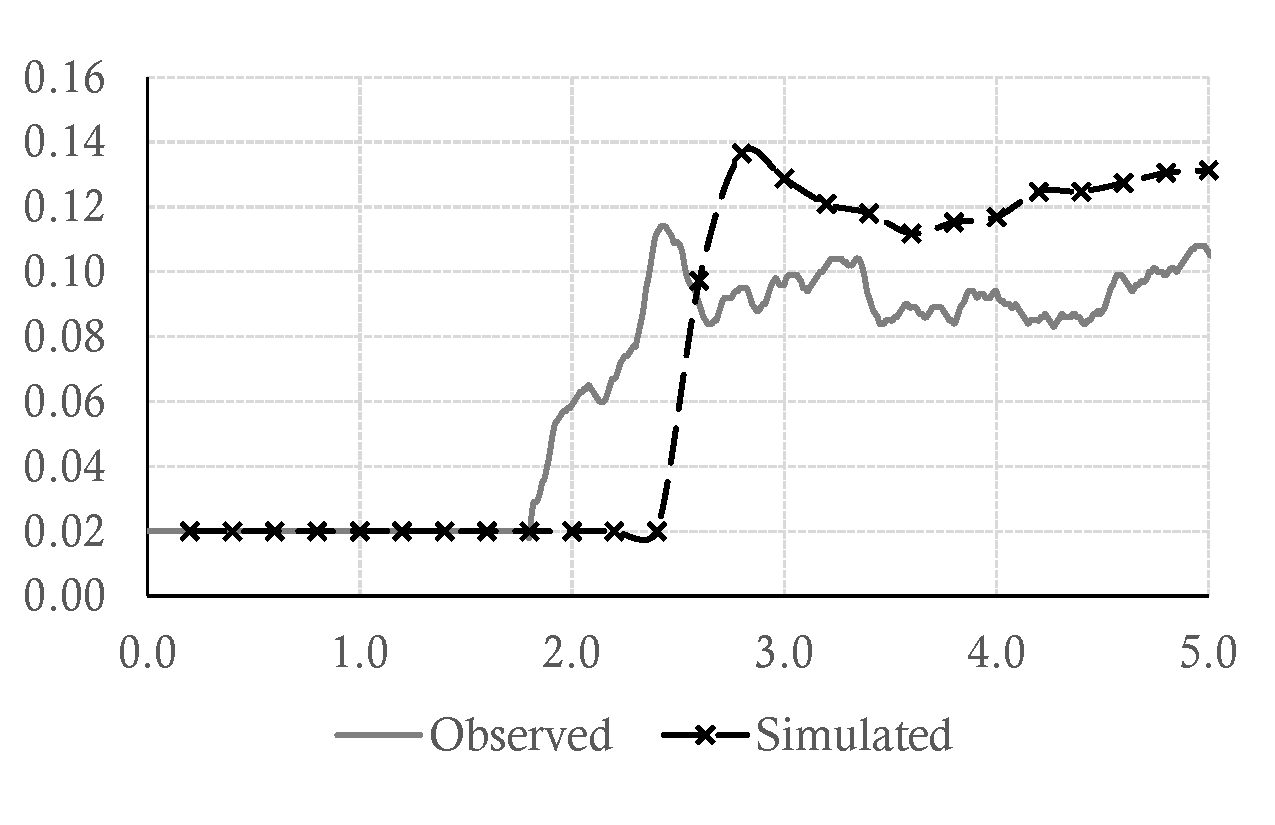
\includegraphics[width=0.5\textwidth]{numerical-test-figures/dam-break-obstacle-results-g3.pdf} &
		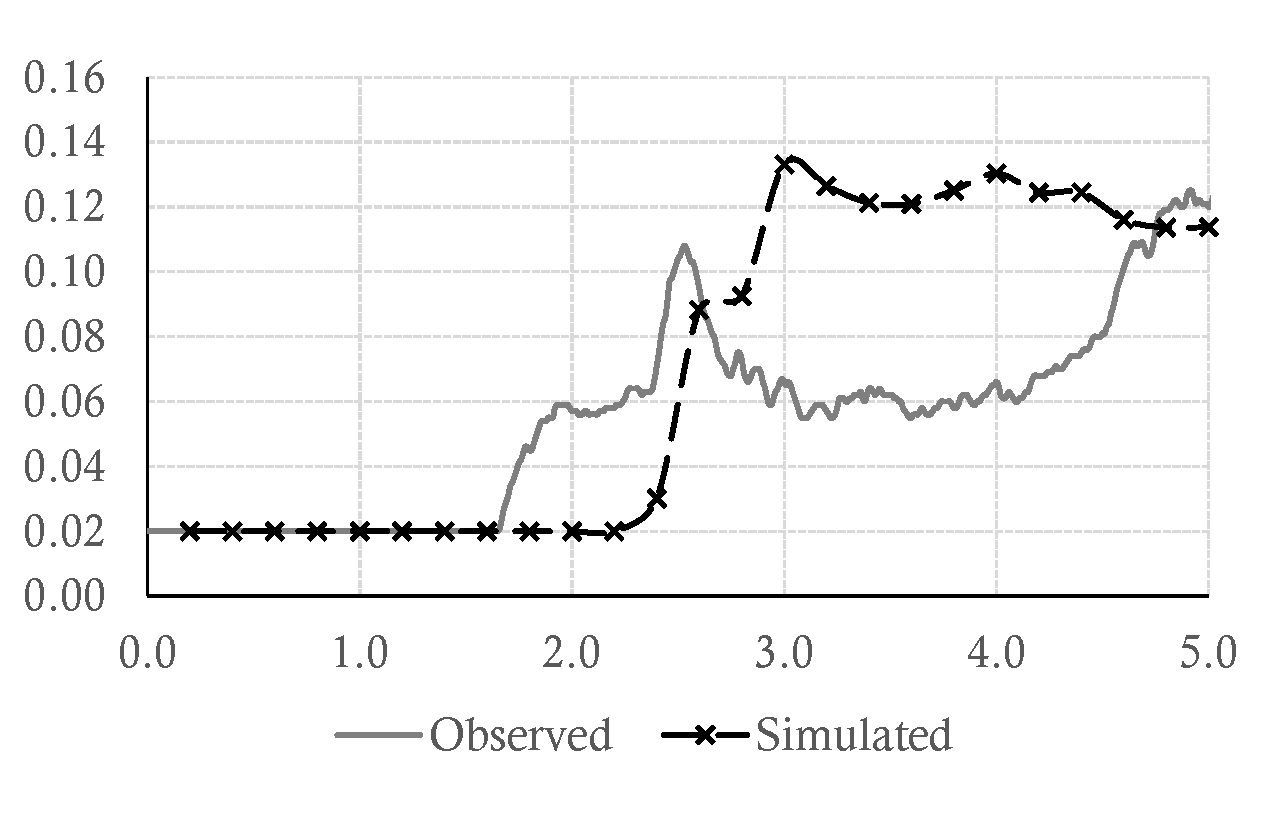
\includegraphics[width=0.5\textwidth]{numerical-test-figures/dam-break-obstacle-results-g4.pdf} \\
		(c) G3 &
		(d) G4 \\[6pt]
		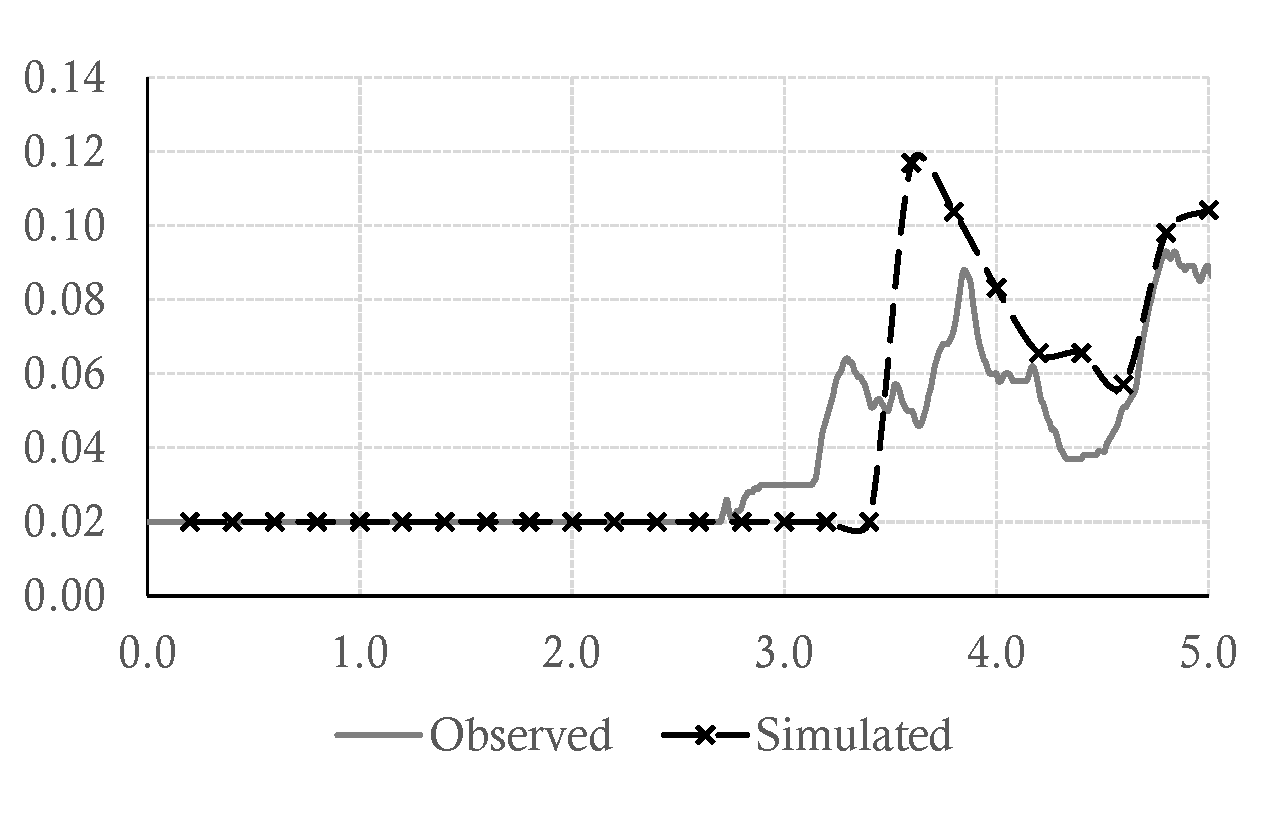
\includegraphics[width=0.5\textwidth]{numerical-test-figures/dam-break-obstacle-results-g5.pdf} &
		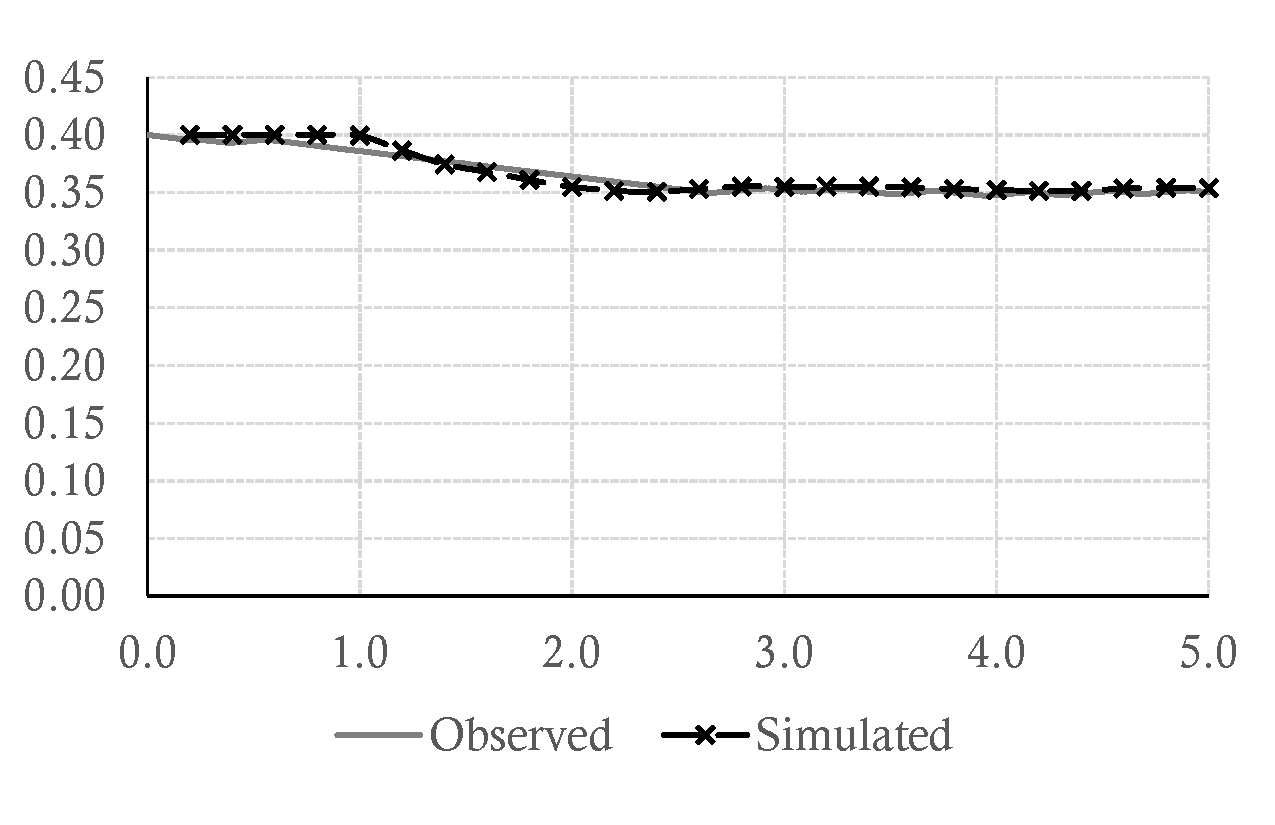
\includegraphics[width=0.5\textwidth]{numerical-test-figures/dam-break-obstacle-results-g6.pdf} \\
		(e) G5 &
		(f) G6 \\
	\end{tabular}
	\caption{Depth comparison between laboratory gauges and simulated results during the first five seconds.}
	\label{TestResult_DamObstacle_Gauges}
\end{figure*}

\section{Hypothetical pluvial flood event}

The previous results provided suggest second-order solutions are required in a wide variety of cases, to avoid significant deviations from the correct result as a consequence of numerical diffusion. Herein, a realistic scenario is considered, of a hypothetical pluvial flood event caused by intense rainfall, within a real-world domain.

The UK Environment Agency commissions a report periodically examining the differences in results, suitability and performance of different 2D hydraulic modelling packages. One of the more complex test-cases therein is a short hypothetical flood event occurring as a combination of both a point inflow and uniform precipitation in the area surrounding Cockenzie Street, Glasgow. The test was performed in accordance with \citet{Pender2010} and \citet{Pender2013}, simulating a 5-hour period.

The inflow hydrograph and hyetograph are given in Figure \ref{Glasgow_Inflows}. The digital terrain model (DTM) is shown in Figure \ref{Glasgow_DTM} alongside the location of the point inflow at (264896, 664747). Data was supplied at 0.5m resolution but has been resampled to 2m to allow comparison with published results for other software. The computational domain contains 97,083 cells. A uniform Manning coefficient of 0.05 is used everywhere except for roads and pavements where a value of 0.02 is assigned, to allow direct comparison with the results in \citet{Pender2010}, although it should be recognised each software will implement the treatment of Manning's $n$ in slightly different manners, hence this is a source of uncertainty. Closed boundary conditions are applied around the extremity of the domain. The surcharging sewer hydrograph is implemented by direct addition of volume to the cell, hence with no initial velocity.

\begin{figure*}[tpb]
\centering
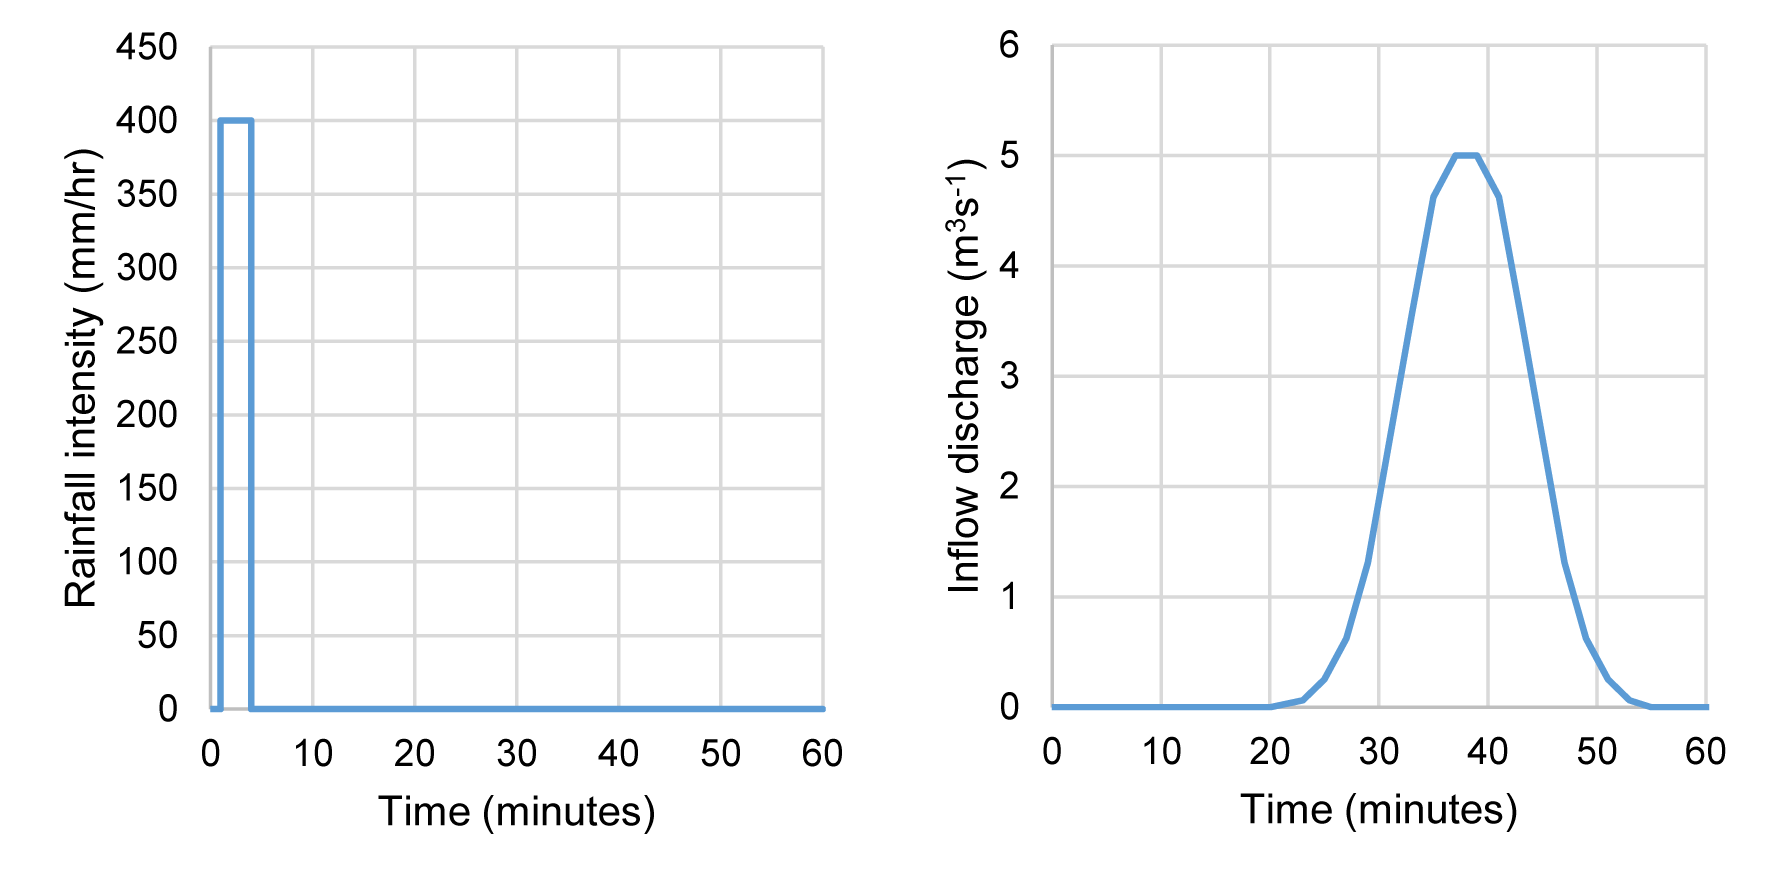
\includegraphics[width=0.75\textwidth]{heterogeneous-dev-figures/Glasgow_Inflow.png}
\caption{Boundary conditions for Glasgow test: (a) Uniformly distributed rainfall hyetograph; (b) volumetric discharge at the inflow point.}
\label{Glasgow_Inflows}
\end{figure*}
\begin{figure*}[tpb]
\centering
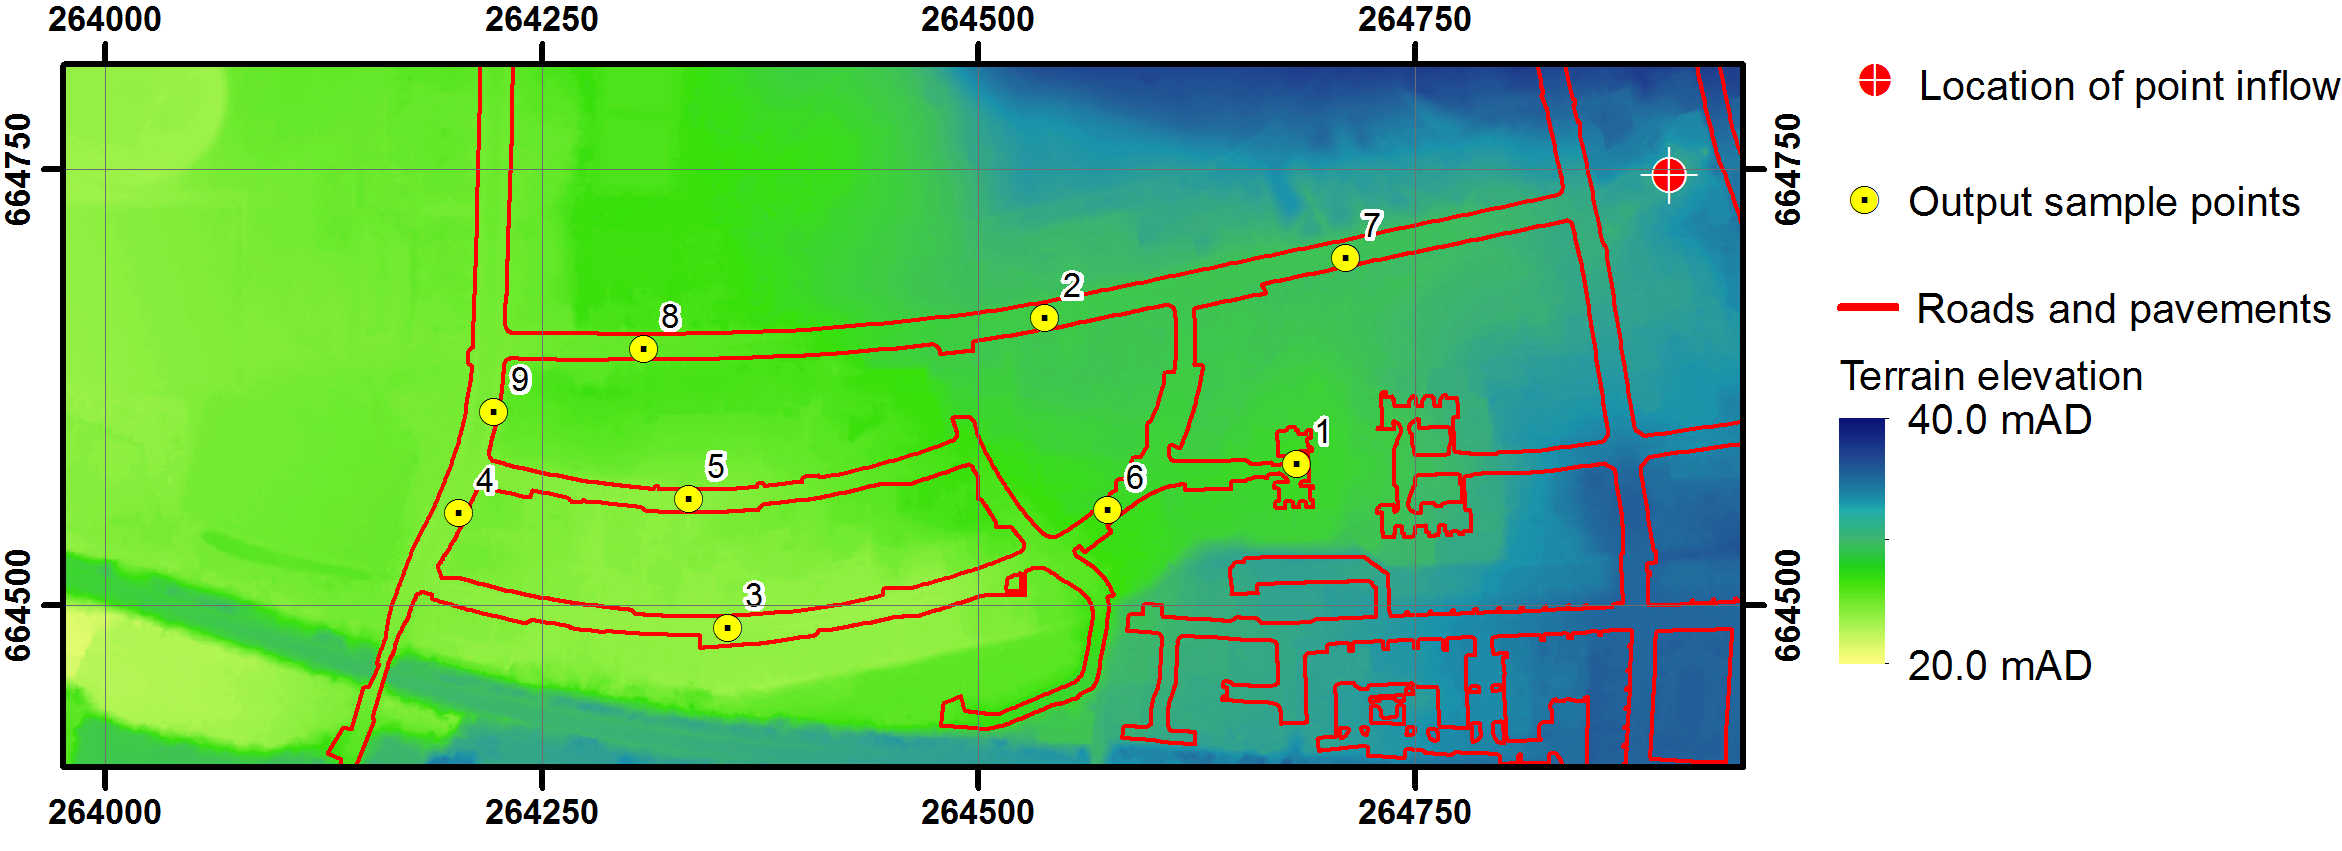
\includegraphics[width=1.0\textwidth]{heterogeneous-dev-figures/Glasgow_DTM.png}
\caption{The surface elevation for a 0.39 km$^{2}$ area of Glasgow with the inflow location indicated and the position of 9 output sample points.}
\label{Glasgow_DTM}
\end{figure*}

Simulations were carried out using 32- and 64-bit floating-point arithmetic (i.e. single- and double-precision). 32-bit arithmetic introduced significant errors (in mass conservation and thus the overall result) for the given numerical scheme, and resulted in timesteps of approximately 0.1s. This is believed to be caused by the lack of numerical resolution for the small depths by which unit-width discharge is divided to give velocities. The typical timestep with 64-bit arithmetic is approximately 0.3s. This difference largely negates the performance benefits that are normally achievable with reduced precision arithmetic for both GPUs and CPUs, and furthermore has implications for any other simulations in which extremely shallow flows might be expected. Results presented hereafter are for 64-bit simulations except where indicated.

The maximum depths recorded per cell at the end of the simulation are displayed in Figure \ref{Glasgow_MaxDepths} at 0.2m intervals. In addition water levels and velocities were output at 9 different points; levels are shown in Figure \ref{Glasgow_PointGraphs} while velocities are omitted for brevity. The maximum depths and timeseries data are consistent with results produced by other software, and close to those of other finite-volume software packages in particular. Small differences are discernible but all fall within the ranges of results presented in \citet{Pender2010}.

\begin{figure*}[tpb]
\centering
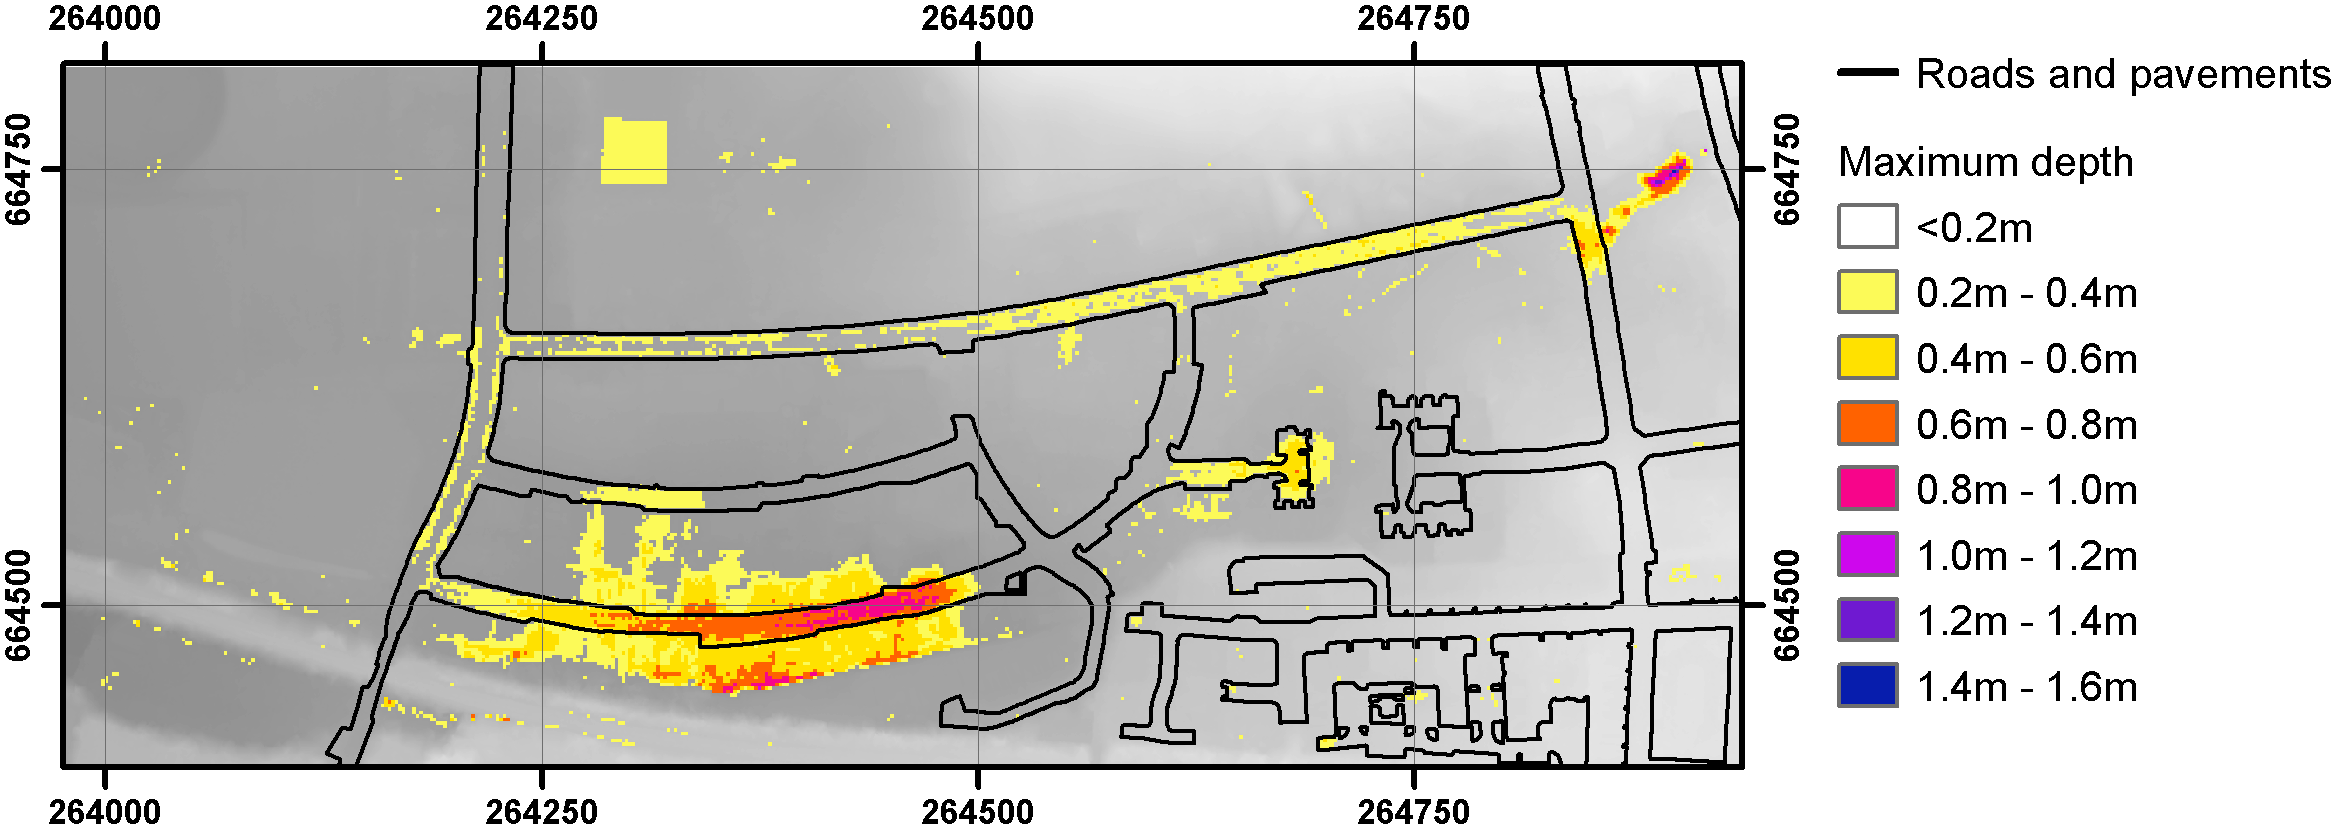
\includegraphics[width=1.0\textwidth]{heterogeneous-dev-figures/Glasgow_MaxDepths.png}
\caption{Maximum water levels observed for the Glasgow test, per cell after 5 hours, shown at 0.2m intervals.}
\label{Glasgow_MaxDepths}
\end{figure*}
\begin{figure*}[tpb]
\centering
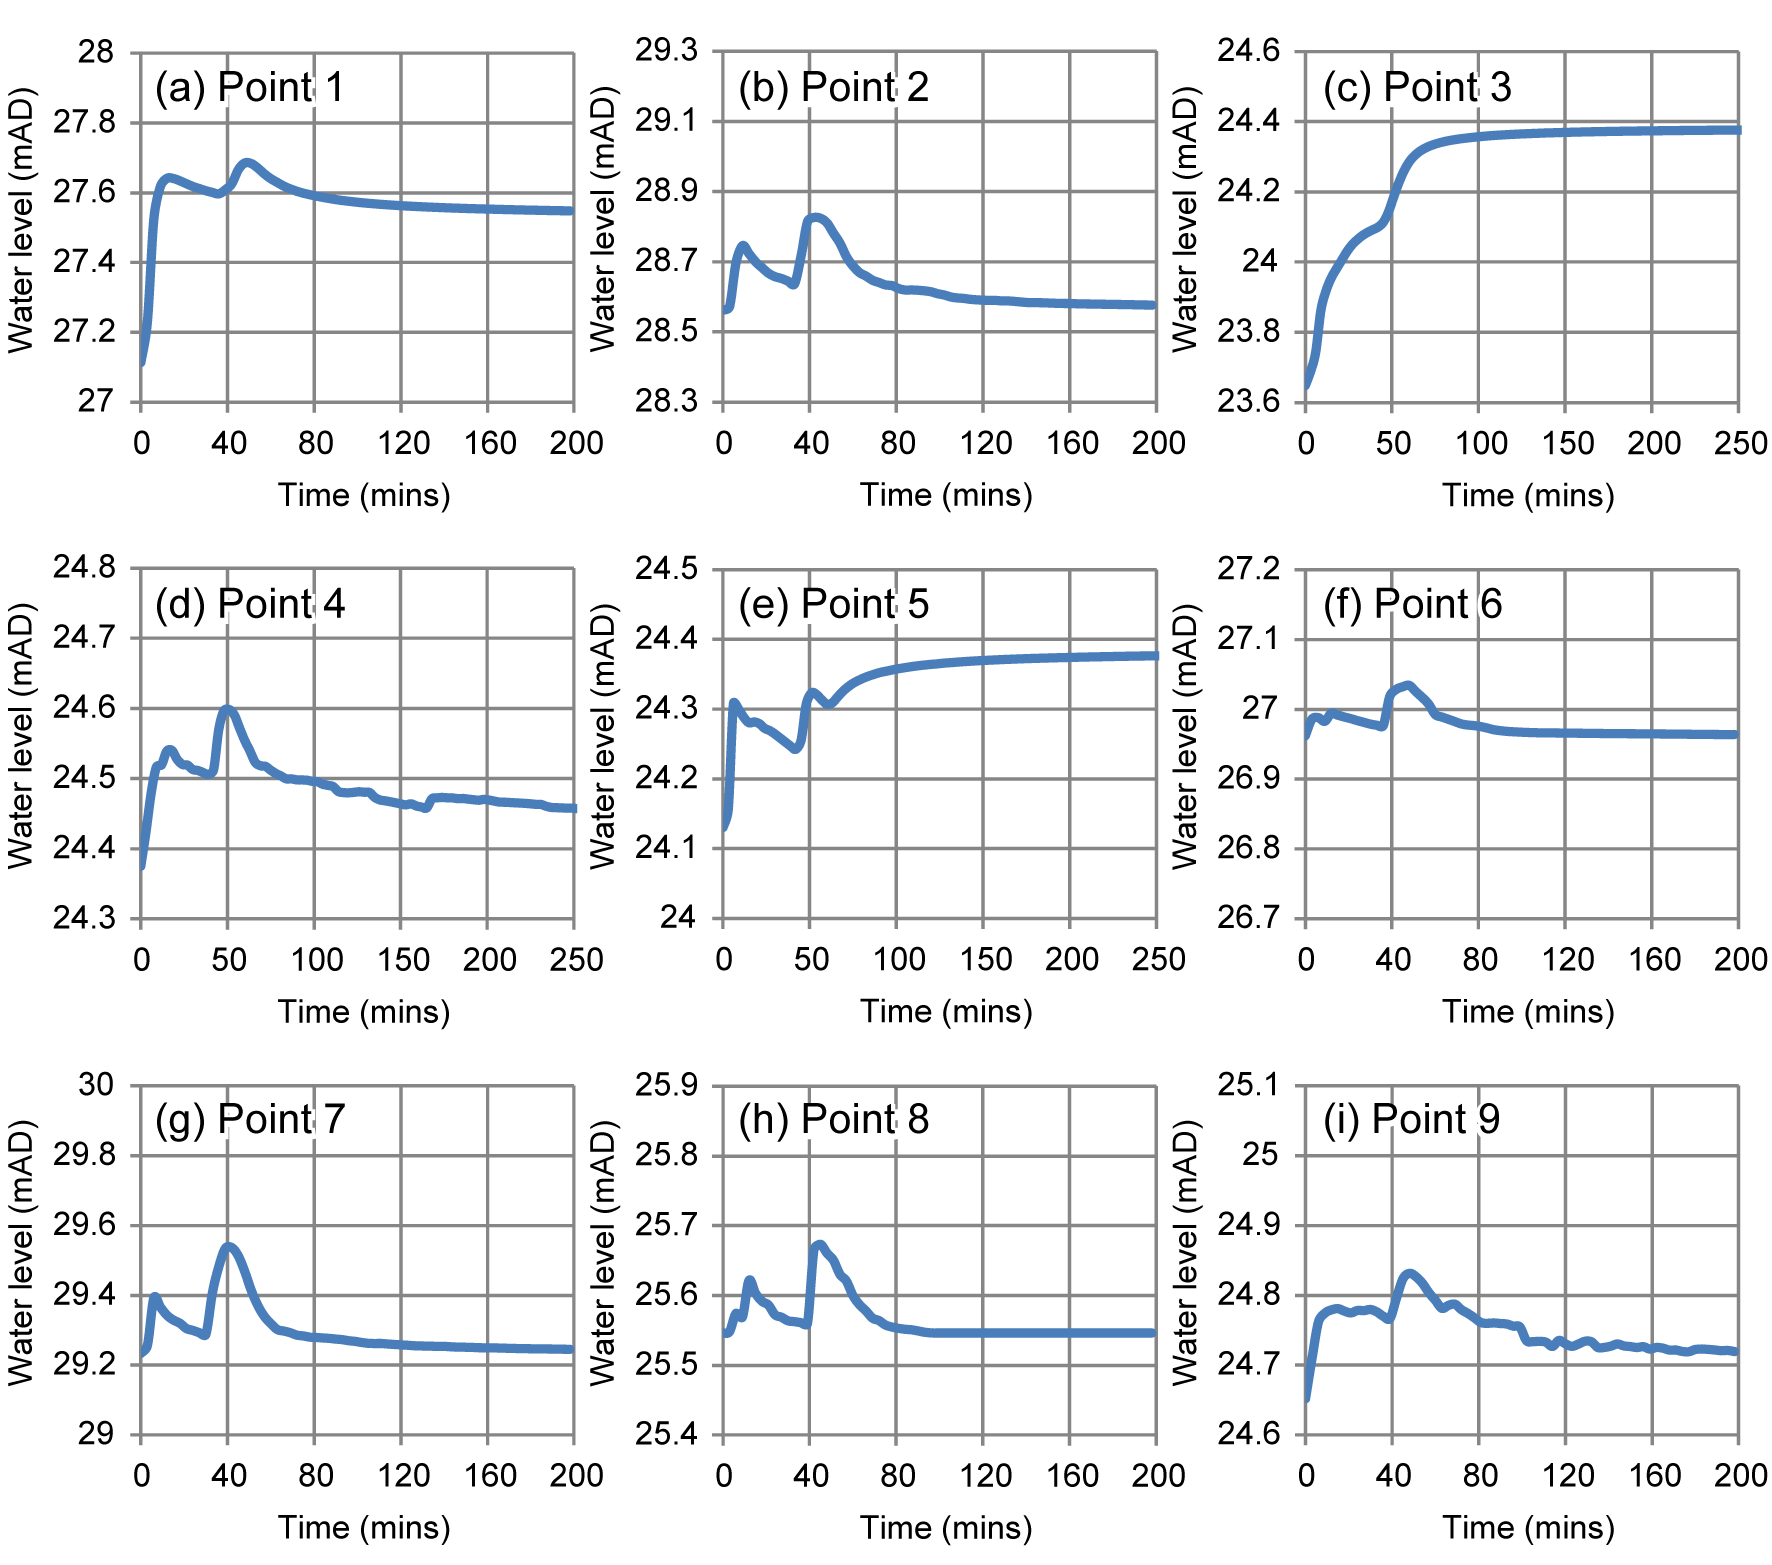
\includegraphics[width=0.8\textwidth]{heterogeneous-dev-figures/Glasgow_PointGraphs.png}
\caption{Changes in recorded water levels for Glasgow, above datum recorded at 9 different sample points in the domain. The location of the sample points is given in Figure \ref{Glasgow_DTM}.}
\label{Glasgow_PointGraphs}
\end{figure*}

The simulation correctly represents the double-peaked nature of the event from intense rainfall and subsequent surcharging of a sewer, with the second peak at point 7 shortly after the surcharging peaked at 38 minutes. The results are generally free of oscillations, except for some small oscillations at point 9 which may be unphysical. At point 2 there is some discrepancy among models as to when the water levels settle after both peaks have passed; the results presented herein suggest this occurs after approximately 120 minutes, which is consistent with the results for the comparable numerical scheme employed in TUFLOW FV. At point 3 the second peak begins at approximately 50 minutes, which is consistent with almost all of the software in \citet{Pender2013}. At point 6 the second peak is predicted to have an elevation around 27.05 mAD, which is higher than many of the other software but there is significant variation across software at this point, ranging from 26.95 to 27.08 mAD. The final flood depths correspond to the areas which were predicted by the majority of software tested in \citet{Pender2013}; clearly a shock-capturing scheme is not necessary to accurately predict the final extent, but can have a marked effect on the progression of the flood wave, localised flow dynamics and arrival timing, all of which could be significant factors in assessing flood risk and crucial in issuing flood warnings. It cannot be asserted as to which software is most accurate as the event and inflow data is hypothetical, however the software herein captures the same behaviour as comparable finite-volume codes solving the full shallow water equations. Small differences in the methods for solving the equations and implementation of boundary conditions can result in significant differences: treatment of wet-dry fronts, frequency of mass addition for precipitation, rounding or smoothing in the consideration of topography, and mechanism for considering the Manning coefficient are believed to be most significant in this instance.

\section{Real-life dam failure at Malpasset (1959)}

The Malpasset dam-break is frequently used as a validation test-case for shock-capturing hydraulic models \citep{Goutal1999}. The double-curvature arch-dam at Malpasset in the south of France failed catastrophically on the 2nd December 1959 at 9:14PM as it approached full capacity during a period of prolonged and intense rainfall. Almost 55,106m\(^{3}\) of water was released downstream towards Fr{\'e}jus, resulting in over 400 deaths. Data is available from a post-event police survey of the extent and a scale model constructed by EDF. The positions of transformers and high-water marks in the valley, plus gauges in the scale model, are indicated in Figure \ref{MalpassetIntro}. A regular Cartesian grid of 10m resolution is used to represent the 18km \(\times\) 10km domain (1.8M cells). The initial free-surface level behind the dam is 100mAD (estimated ±0.5m error), and sea level 0mAD. Comparison of results on the left- and right-hand sides of the valley are presented in Figure \ref{MalpassetValidation} for \(n=0.033\) (\(M=30\)), the value suggested by CADAM project participants.  The first 4000 seconds following the collapse are simulated.

Figure \ref{MalpassetProgression} shows the inundation extent in the valley at \(t=1000\), \(t=2000\), \(t=3000\), and \(t=4000\) seconds. The final extent and agreement with the police survey are consistent with other studies such as \citet{Brodtkorb2011}, with a larger range of parametric sensitivity nearest the dam site. The suggest Manning value is not guaranteed to be transferable between different numerical models and spatial discretisations, but in all instances the police survey falls within the range of parameterisations tested.

\begin{figure*}[tpb]
\centering
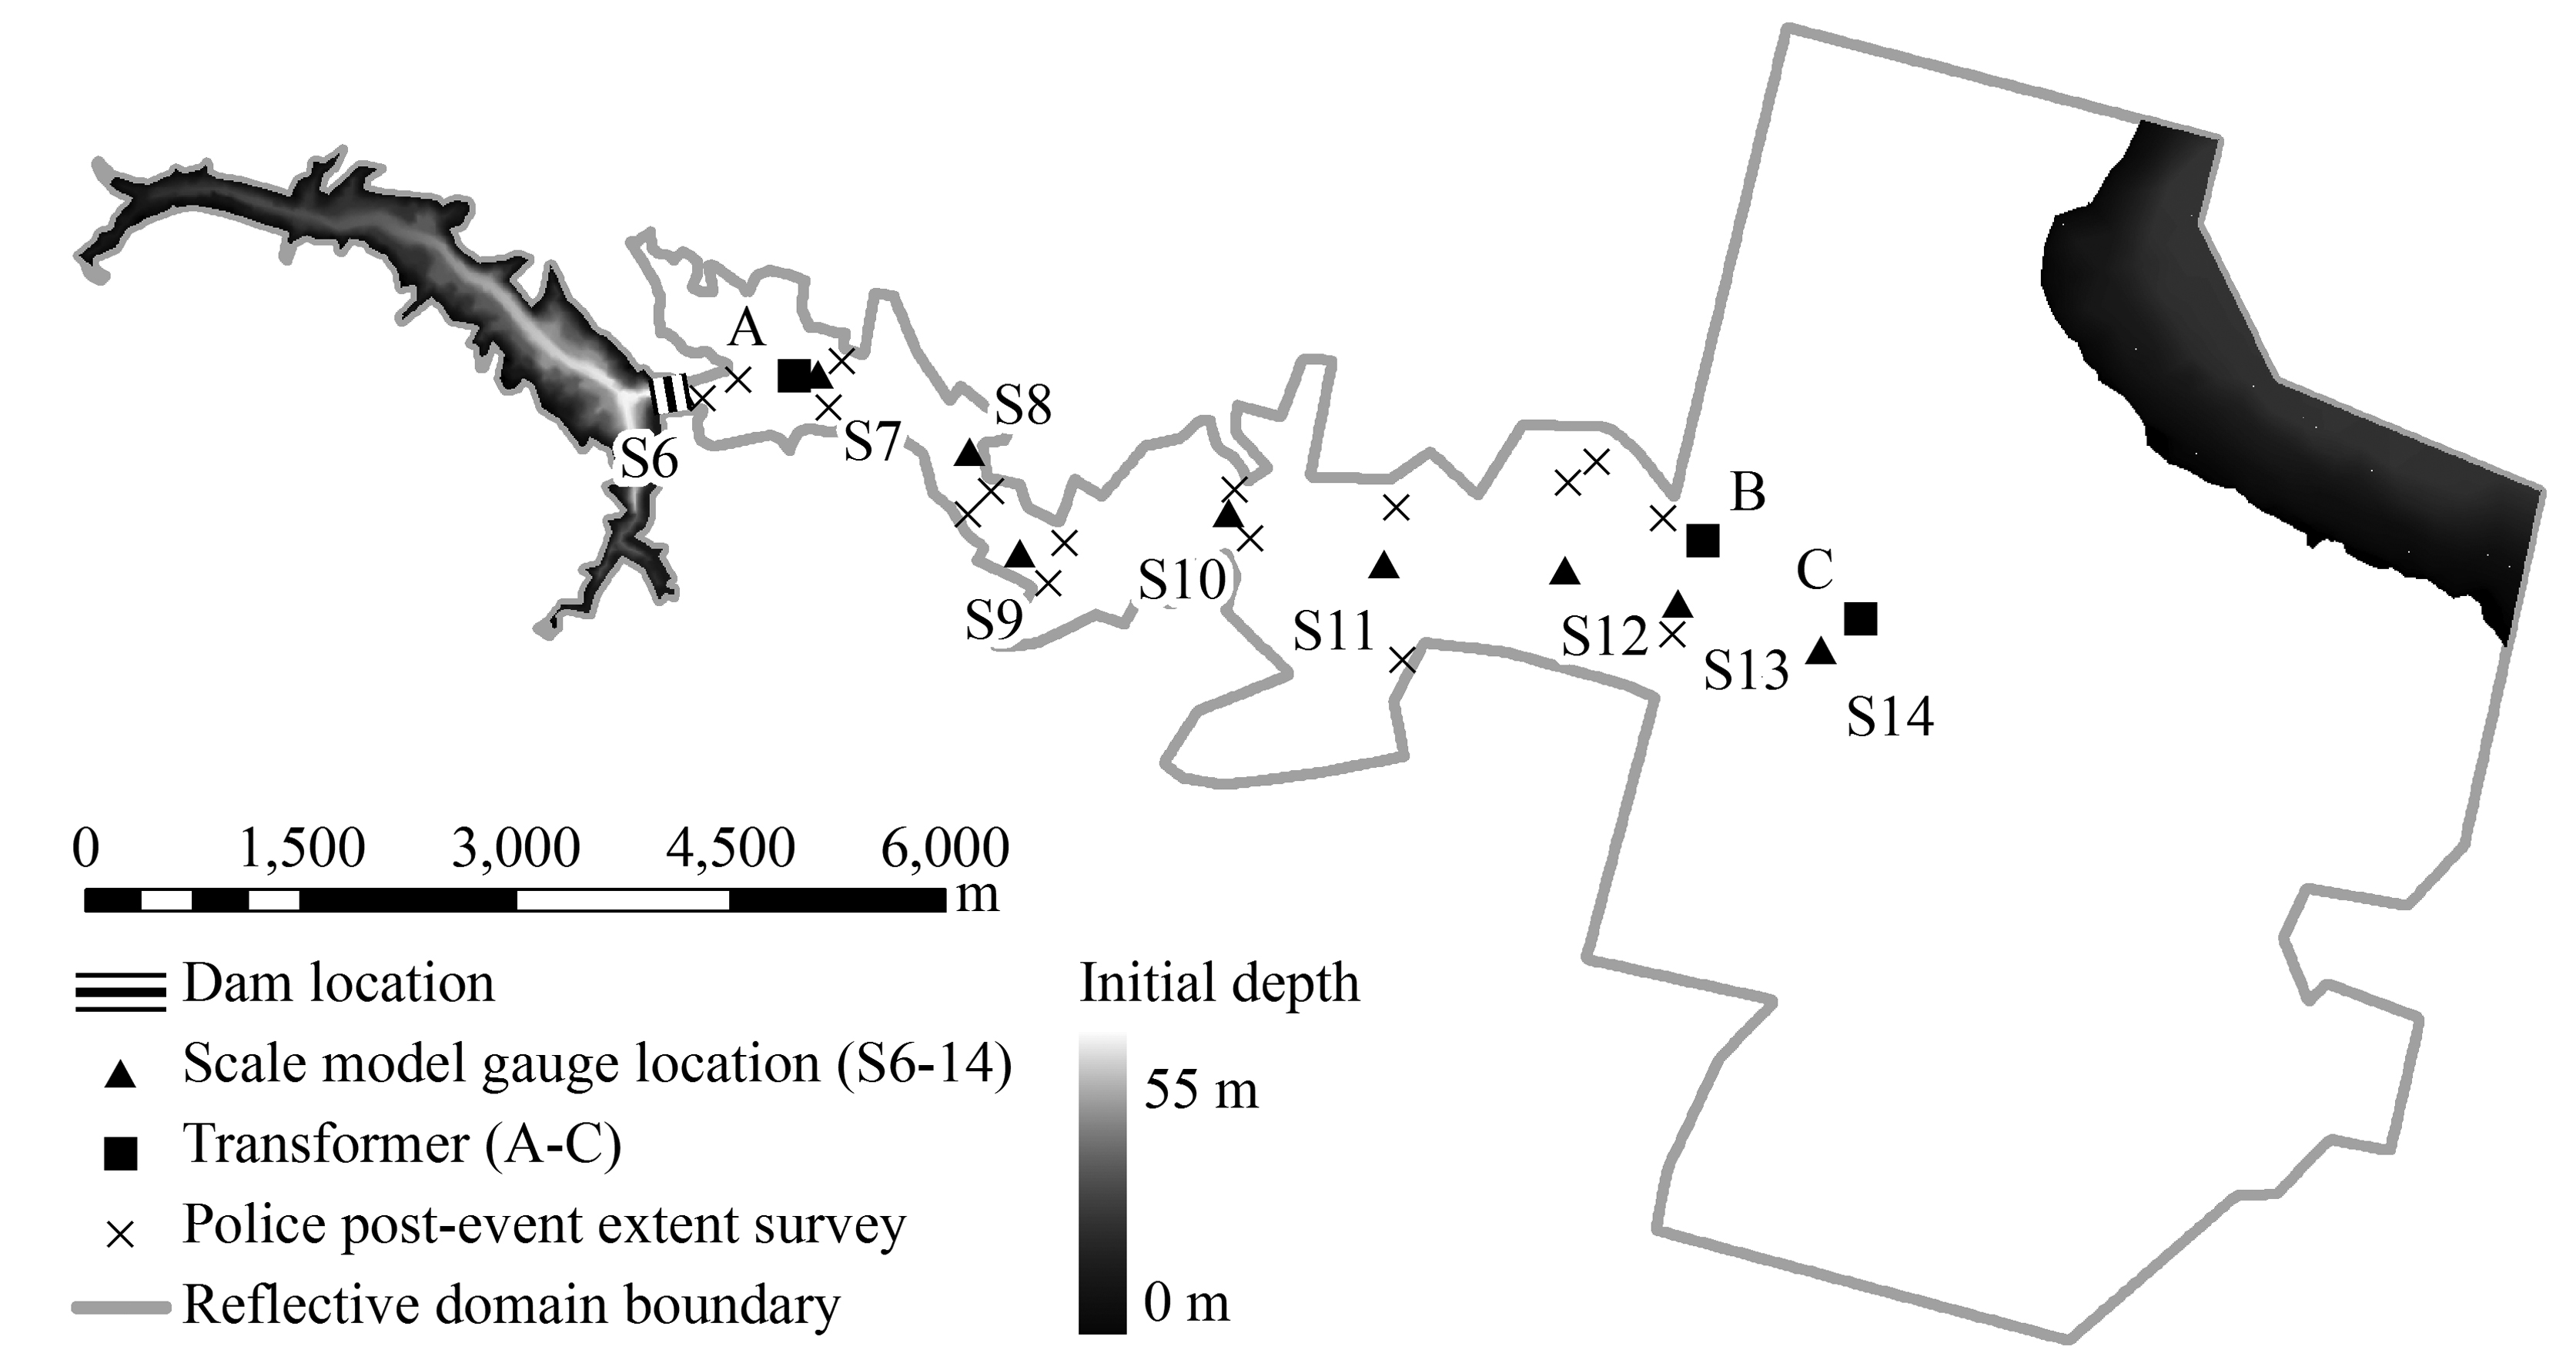
\includegraphics[width=1.0\textwidth]{heterogeneous-dev-figures/Figure_8_Greyscale.jpg}
\caption{Malpasset dam-break domain, initial conditions and locations of validation points.}
\label{MalpassetIntro}
\end{figure*}
\begin{figure*}[tpb]
\centering
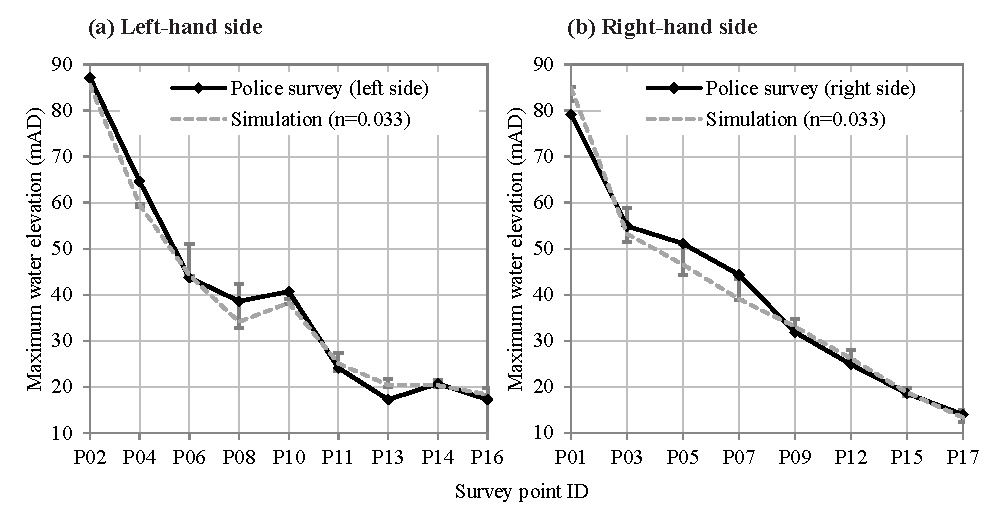
\includegraphics[width=1.0\textwidth]{heterogeneous-dev-figures/Figure_10_Greyscale.pdf}
\caption{Comparison of maximum simulated free-surface levels in Malpasset, on the left- and right-hand sides of the valley (looking downstream) against post-event police survey. Error bars indicate results for $0.022 \le n \le 0.100$ }
\label{MalpassetValidation}
\end{figure*}
\begin{figure*}[tpb]
\centering
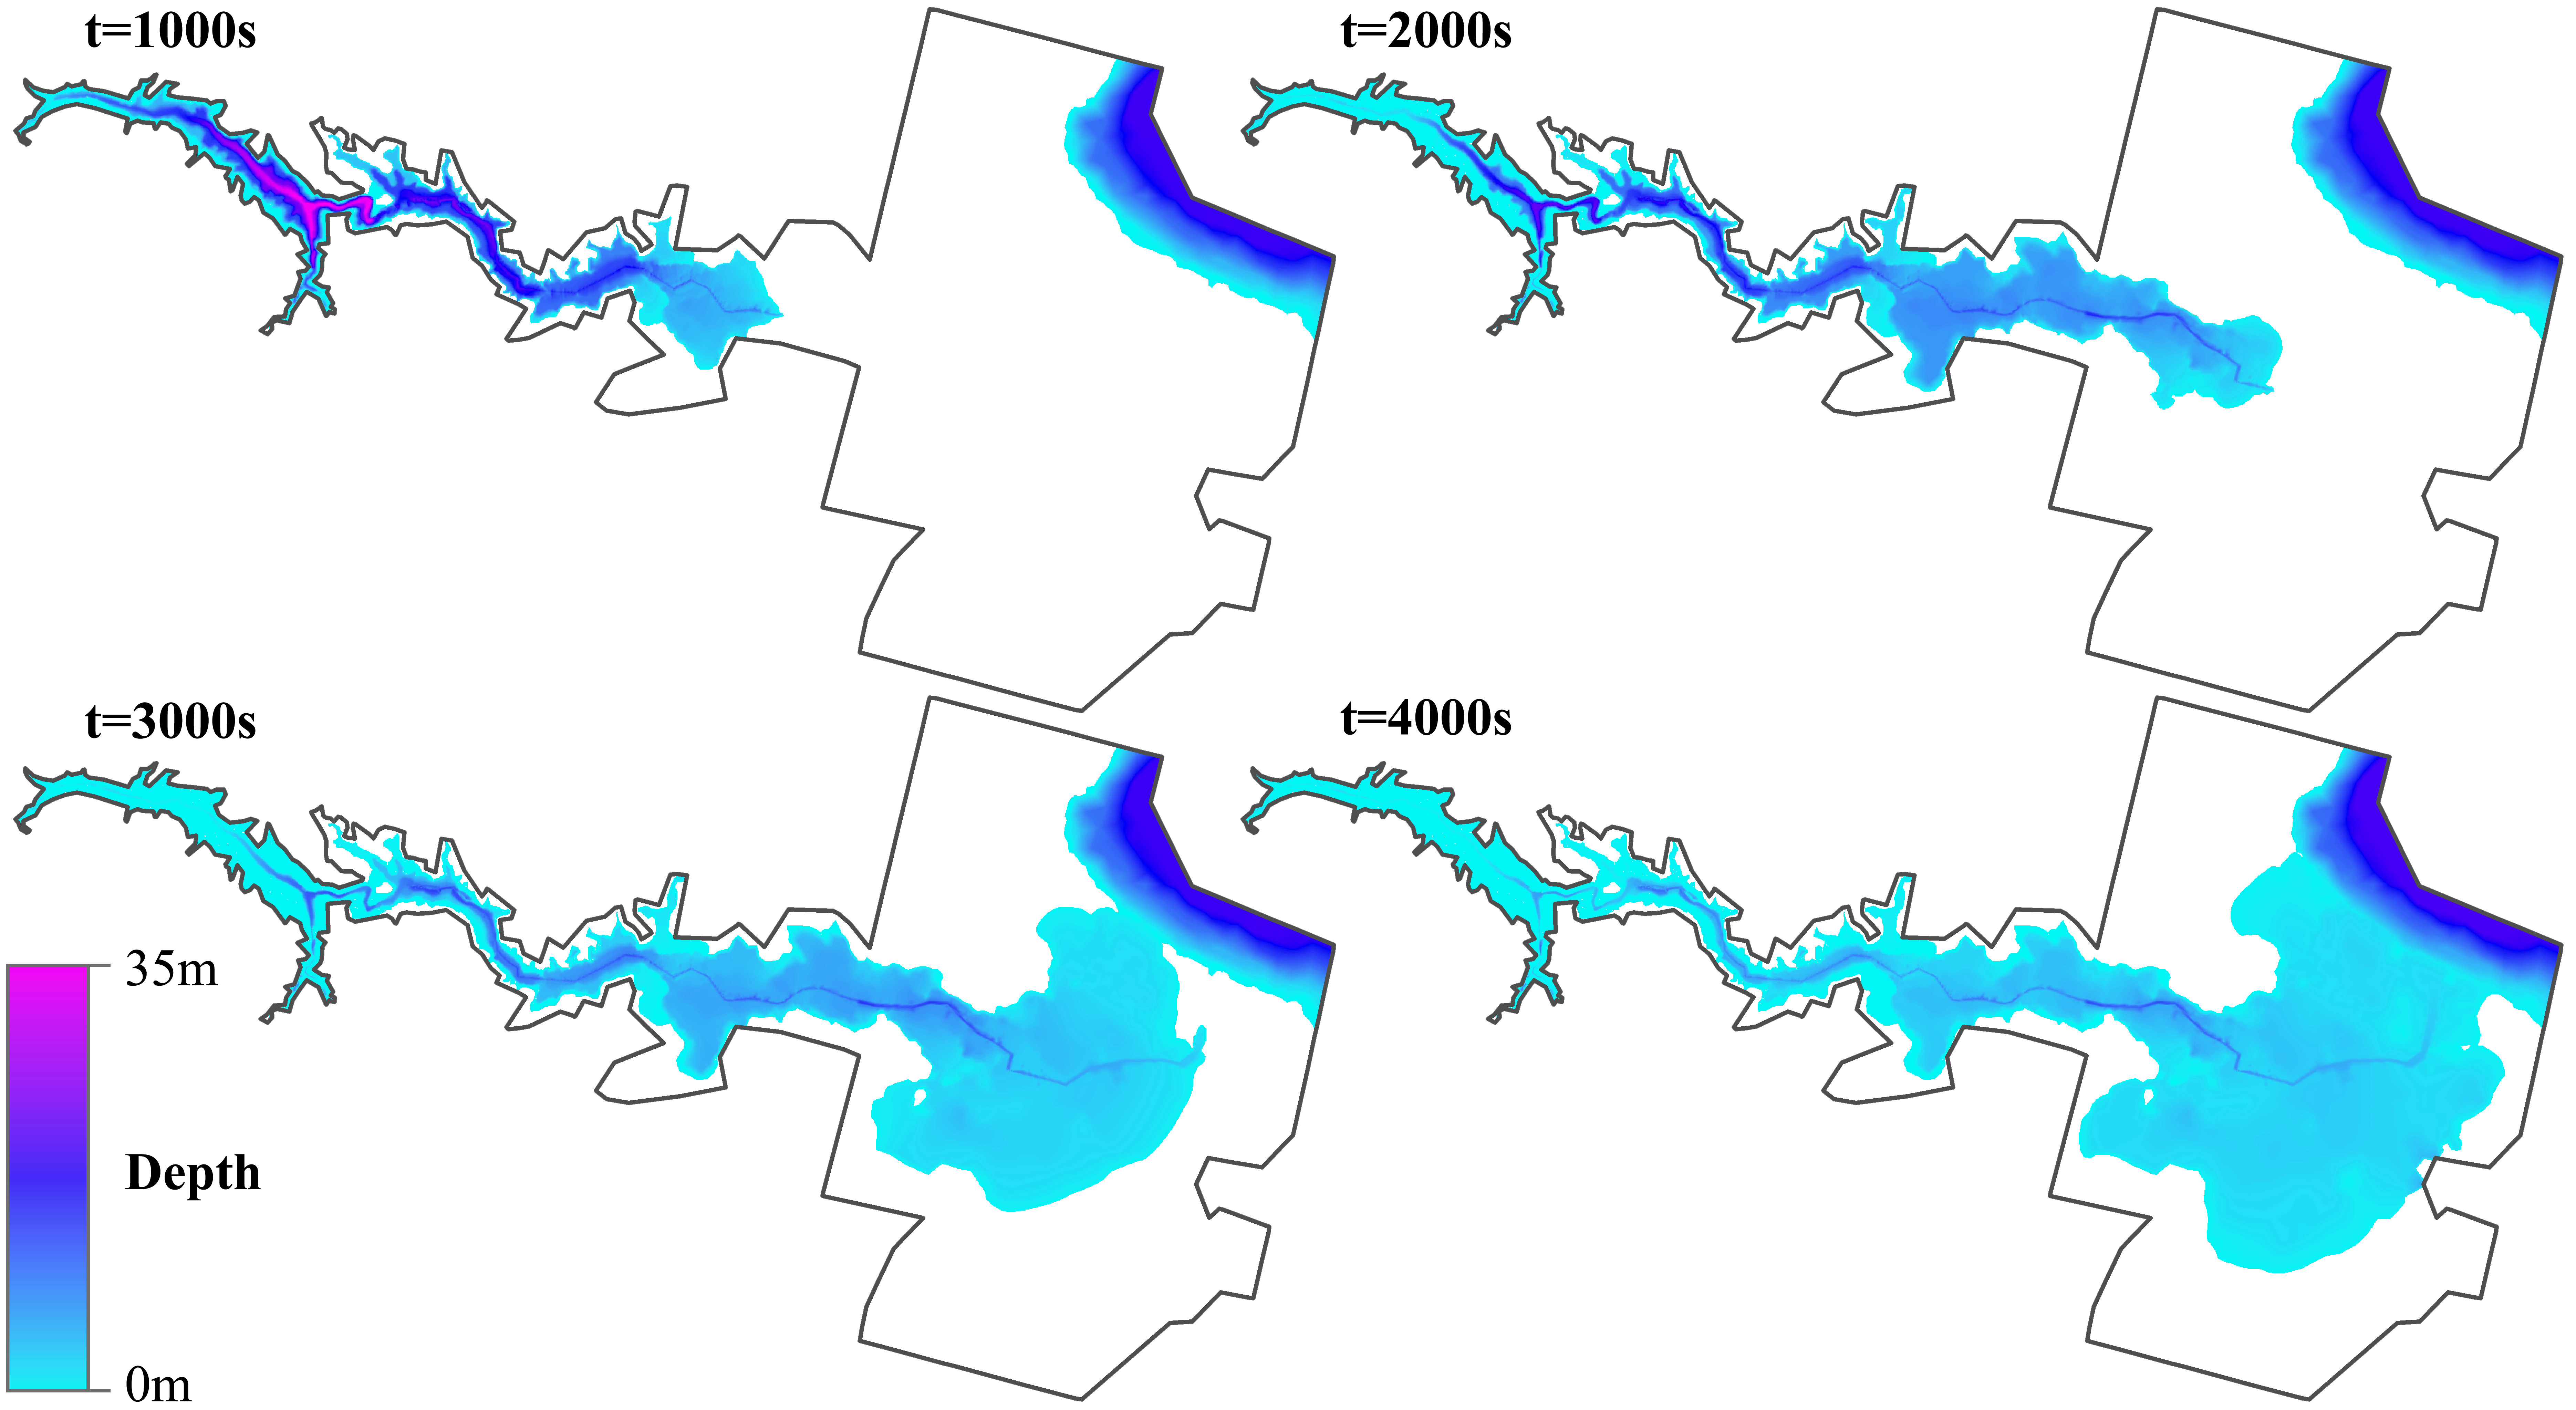
\includegraphics[width=1.0\textwidth]{heterogeneous-dev-figures/Figure_9_Colour.jpg}
\caption{Evolving inundation map for the Malpasset valley every 1000 seconds.}
\label{MalpassetProgression}
\end{figure*}

\section{Computational performance}

The tests at the beginning of this chapter were intended and designed to establish the accuracy of the simulation results, and the suitability for different flow scenarios. The later tests are more suited to performance comparison, as they represent real-world of similar situations. The second-order scheme requires more intensive computation, and it naturally follows that run-times will be longer. Whether the accuracy benefits are justified in the context of longer simulation run-times, is likely to be case dependent and no simple matter. Further performance gains can be achieved by reducing the precision of the calculations, using 32-bit floating-point arithmetic in place of 64 bits. The compound effect of this reduced precision is also discussed here.

\subsection{First-order Godunov-type scheme}

\begin{table*}[pb]
\newcolumntype{R}[1]{>{\RaggedLeft\arraybackslash}p{#1}}
\small
\centering
\caption{Simulation run-times for Glasgow in minutes using three different processing devices.}
\label{GlasgowPerformance}
\begin{tabular}{p{0.15\textwidth}R{0.15\textwidth}R{0.15\textwidth}R{0.15\textwidth}}
\hline
\raggedright{Floating-point arithmetic resolution}	& CPU Intel Xeon E5-2609 & GPU AMD FirePro V7800 		& GPU NVIDIA Tesla M2075 \\
\hline
32-bit 							& 9.05					& 2.47					& 1.98				\\
64-bit 							& 9.45					& 2.67					& 2.88				\\
\hline
\end{tabular}
\end{table*}

The run-times for the Glasgow simulation described earlier in this chapter, using three different processing devices are presented in Table \ref{GlasgowPerformance}. It is important to note however that the domain for this test-case is too small to fully exploit the weak scaling in GPUs. Nonetheless the times represent a significant reduction on those in \citet{Pender2010} and \citet{Hunter2007}, with both CPU and GPU computation, despite the use of an explicit numerical scheme and Godunov-type scheme.

The CPU results are broadly as expected. GPUs however, are designed with 32-bit computation as their primary purpose. The AMD GPU should exhibit inferior performance to the NVIDIA Tesla, according to the device specifications. The disparity can likely be attributed to the overheads, and not providing a suitably large domain to fully leverage these devices.

Compared to figures reported for the same test in \citet{Pender2013}, the software presented herein is slightly slower than some comparable GPU software (e.g. 1.40 minutes for TUFLOW GPU), which may in part be a result of using OpenCL parallelisation, where there is some evidence to suggest memory transfers and dispatch overheads could be slightly higher than CUDA \citep[e.g.][]{Karimi2010}. The performance results cannot be directly compared however as different hardware was used for each software. Moreover, the CUDA and OpenCL APIs have subtle but important differences between implementations, such as the non-standard blocking behaviour of \texttt{clEnqueueNDRangeKernel} in NVIDIA's implementation of OpenCL, where a call scheduling work on the GPU will not return until the work is complete, making it impossible to queue many iterations of the numerical scheme to reduce the launch overhead. Comparison is also difficult as diffusion approximation codes \citep[e.g.][]{Bates2000} can be expected to exhibit poor computational efficiency at 2m resolution because of a more severe timestep constraint.

\subsection{Second-order MUSCL-Hancock scheme}

\begin{table*}[tb]
	\small
	\centering
	\caption{Total simulation time and cell calculation rate using three different devices, cache configurations and floating-point precisions, for the Malpasset dam failure second-order simulation. The kernel and cache configurations are described in Chapter \ref{chapter:NumericalMethods} and Figure \ref{Kernels}.}
	\label{Malpasset_PerformanceResults}
	\begin{tabular}{llrrrrrr}
		\hline
		& 			& \multicolumn{2}{c}{AMD FirePro V7800}			& \multicolumn{2}{c}{NVIDIA Tesla M2075}			& \multicolumn{2}{c}{Intel Xeon E5-2609} 	\\
		Kernels/cache 		& Precision 	& \begin{tabular}[t]{@{}c@{}}Time \\ (s)\end{tabular} 	& \begin{tabular}[t]{@{}c@{}}Rate \\ (x10\textsuperscript{6}/s)\end{tabular} 	& \begin{tabular}[t]{@{}c@{}}Time \\ (s)\end{tabular} 	& \begin{tabular}[t]{@{}c@{}}Rate \\ (x10\textsuperscript{6}/s)\end{tabular}	& \begin{tabular}[t]{@{}c@{}}Time \\ (s)\end{tabular} 	& \begin{tabular}[t]{@{}c@{}}Rate \\ (x10\textsuperscript{6}/s)\end{tabular} 	\\
		\hline
		A: None 				& 32-bit 		& 84 			& 435	 		& 66 			& 556	 		& 821 		& 45	 \\
		& 64-bit 		& 363 		& 106	 		& 243 		& 159	 		& 1534 		& 25	 \\
		B: Normal				& 32-bit 		& 142 		& 258	 		& 125 		& 294	 		& 956 		& 38	 \\
		& 64-bit 		& 446 		& 86		 		& 381 		& 101	 		& 1730 		& 22	 \\
		B: Oversized			& 32-bit 		& 122 		& 300	 		& 88 			& 417	 		& 951 		& 39	 \\
		& 64-bit 		& 442 		& 87		 		& 366 		& 105	 		& 1739 		& 22	 \\
		C: Normal				& 32-bit 		& 122 		& 298	 		& 117 		& 314	 		& 1136 		& 32	 \\
		& 64-bit 		& 844 		& 45		 		& 576 		& 67		 		& 2818 		& 14	 \\
		C: Oversized			& 32-bit 		& 110 		& 335	 		& 88 			& 417	 		& 1144 		& 32	 \\
		& 64-bit 		& 820 		& 47		 		& 554 		& 69		 		& 2881 		& 13	 \\
		\hline
	\end{tabular}
\end{table*}

The run-times with multiple configurations of the software developed herein are presented in Table \ref{Malpasset_PerformanceResults} for the different hardware used to simulate the Malpasset event. The results indicate that for 64-bit computation the NVIDIA GPU model can simulate the Malpasset collapse 6.3$\times$ faster than the Intel CPU, while the manufacturer-quoted peak performances suggest a 6.7$\times$ difference \citep{NVIDIACorporation2011,IntelCorporation2012}; the actual and and quoted performance differences for the AMD device are 4.2 and 5.2 respectively \citep{AMD2012}. This is not altogether surprising; further analysis suggests the AMD device with 64-bit floating-point does not achieve full occupancy because the number of registers constrains the number of AMD wavefronts. Nonetheless the AMD simulation time represents a significant improvement over the CPU, for a fraction of the cost of an NVIDIA Tesla GPU (per Table \ref{CPUGPUCosts}). Vendor-quoted peak performance levels are rarely achievable in practical applications and are compared only to give an indication of device processing power. For users without a suitable GPU the software will nevertheless provide a significant performance boost, given that the new software fully harnesses all four cores of the CPU at all stages of the numerical scheme, unlike most existing commercial software.

Caching data to local memory provides no performance benefit with 32- or 64-bit floating-point computation for any of the devices tested herein. Where local memory is used however, oversizing the array is often shown to improve performance by alleviating bank conflicts, for the reasons previously outlined in Section \ref{Subsection:StorageMemoryHeterogeneous}.

\section{Effects of floating-point precision}

\begin{figure*}[p]
	\centering
	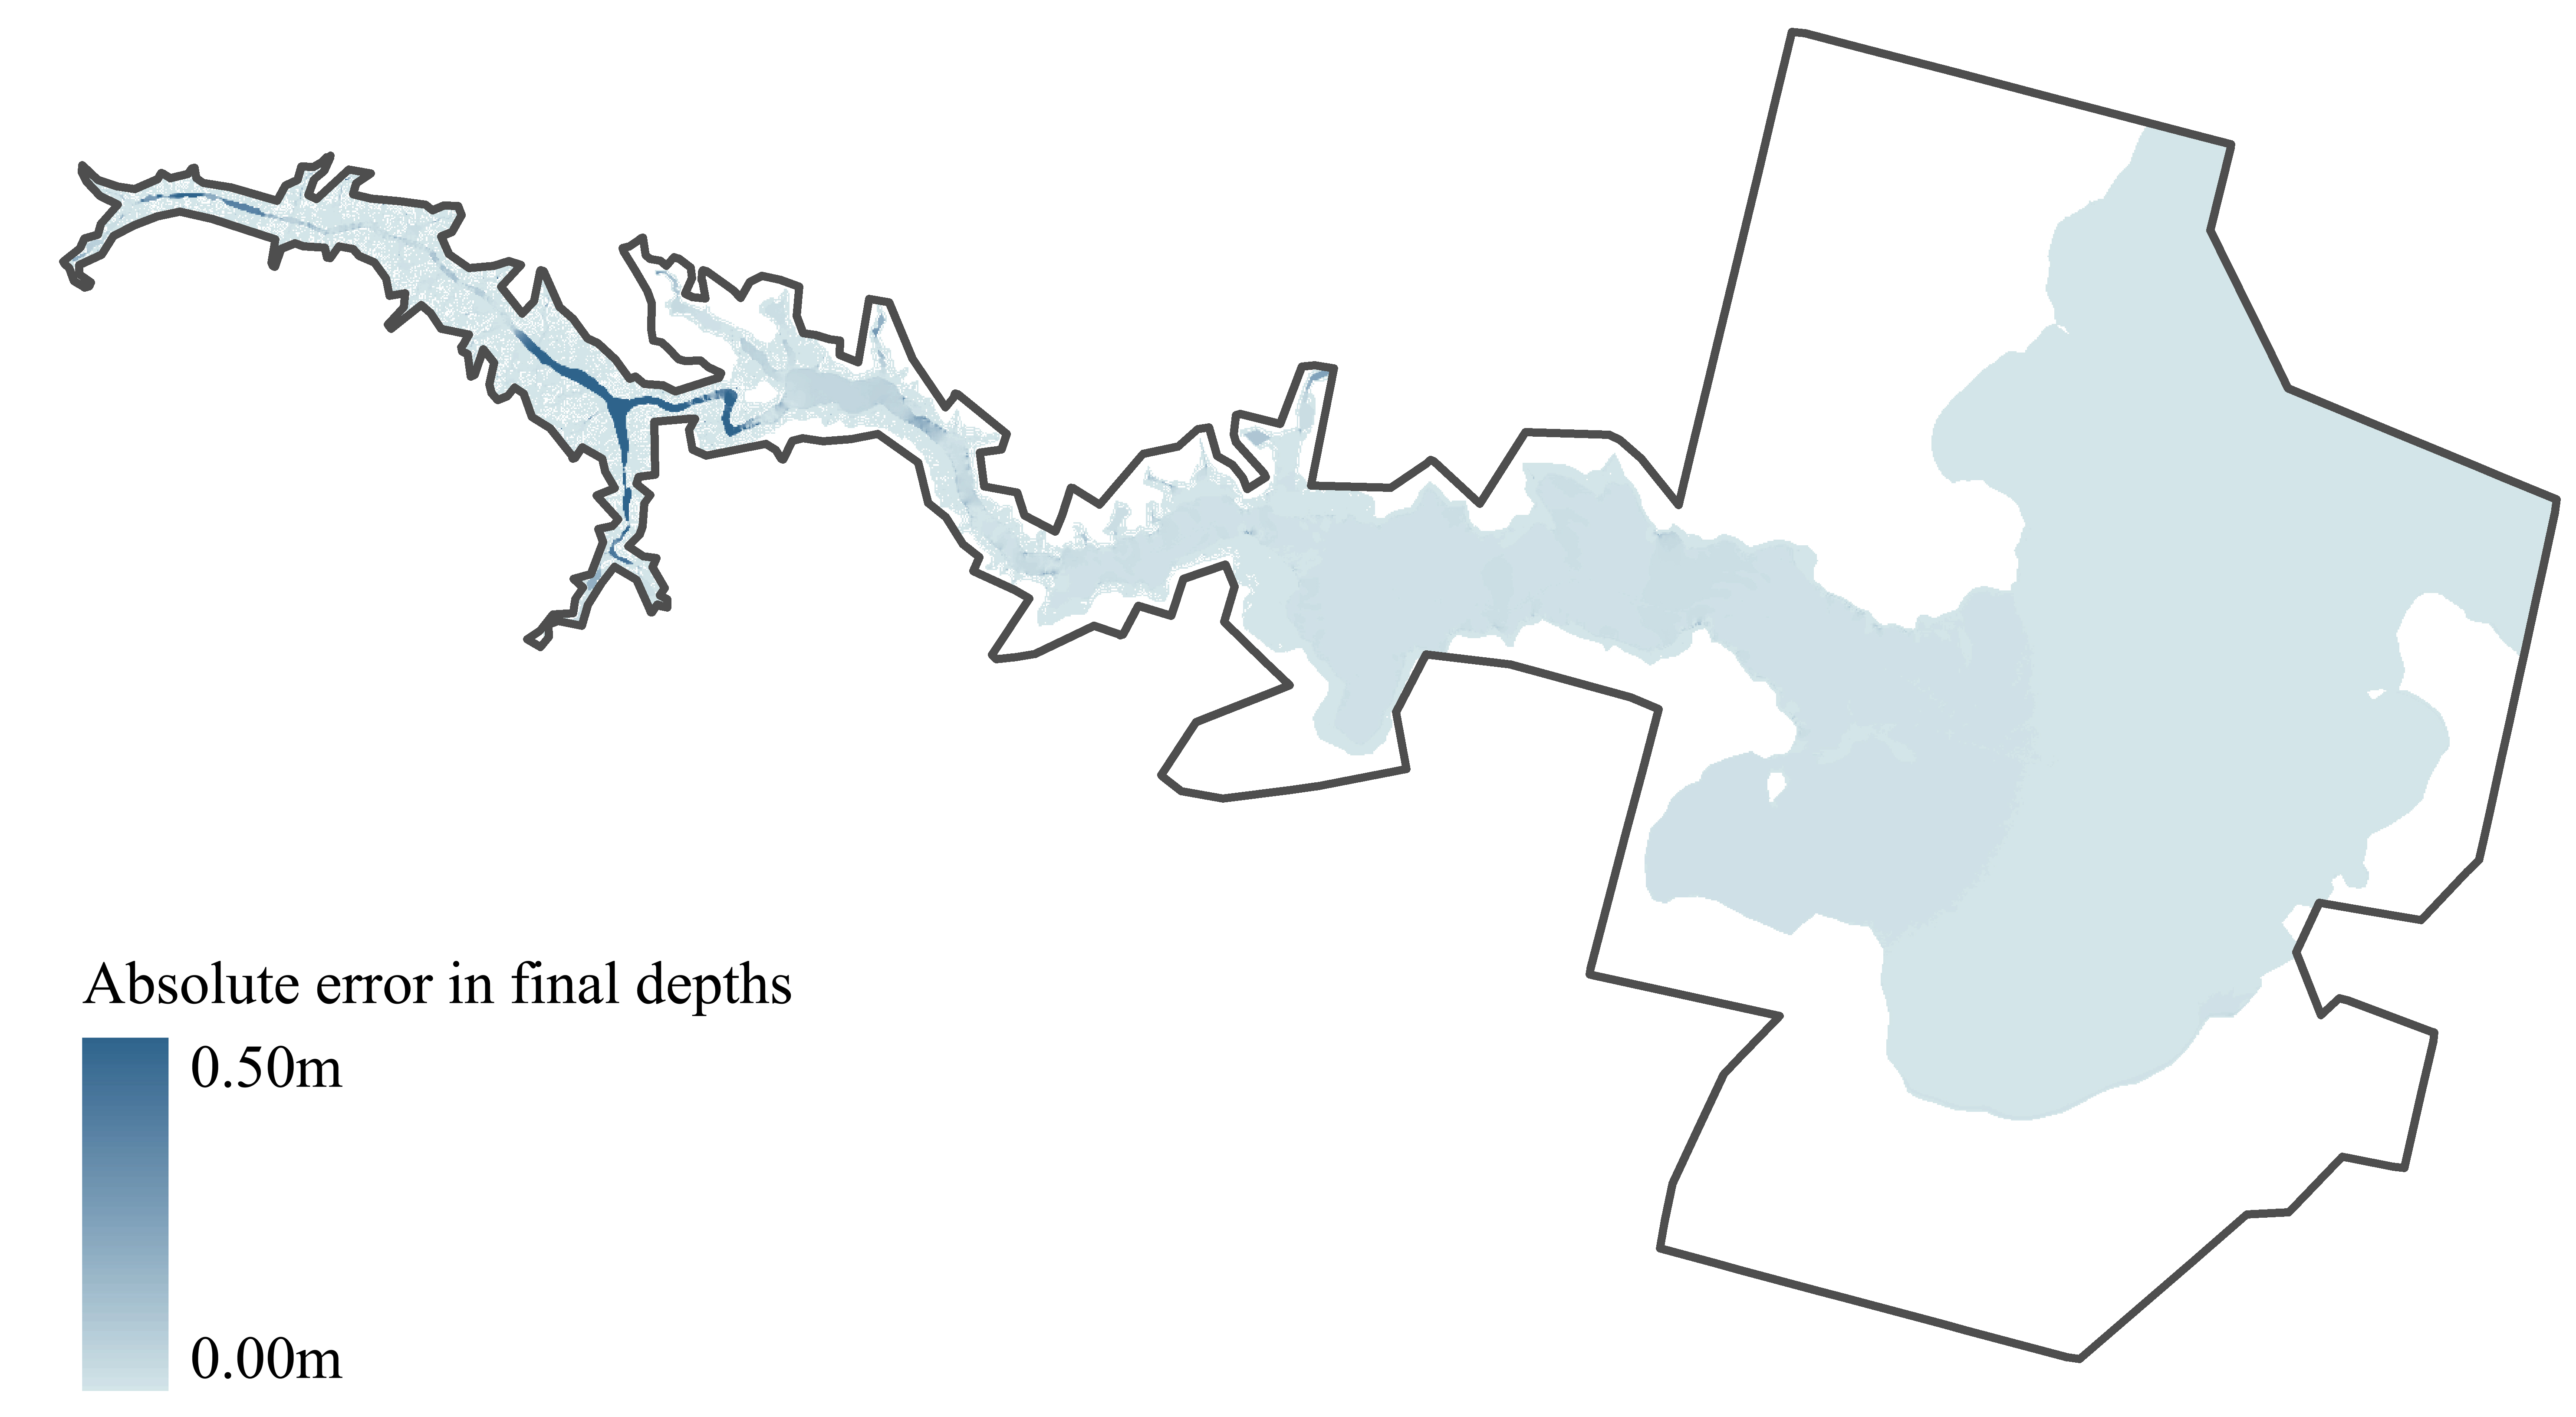
\includegraphics[width=1.0\textwidth]{heterogeneous-dev-figures/Figure_11_Colour.jpg}
	\caption{Spatial distribution of absolute errors in Malpasset, introduced in the final depths (4000s) by using 32-bit floating-point after the Malpasset collapse, when compared to 64-bit results.}
	\label{FPErrorFinal}
\end{figure*}
\begin{figure*}[p]
	\centering
	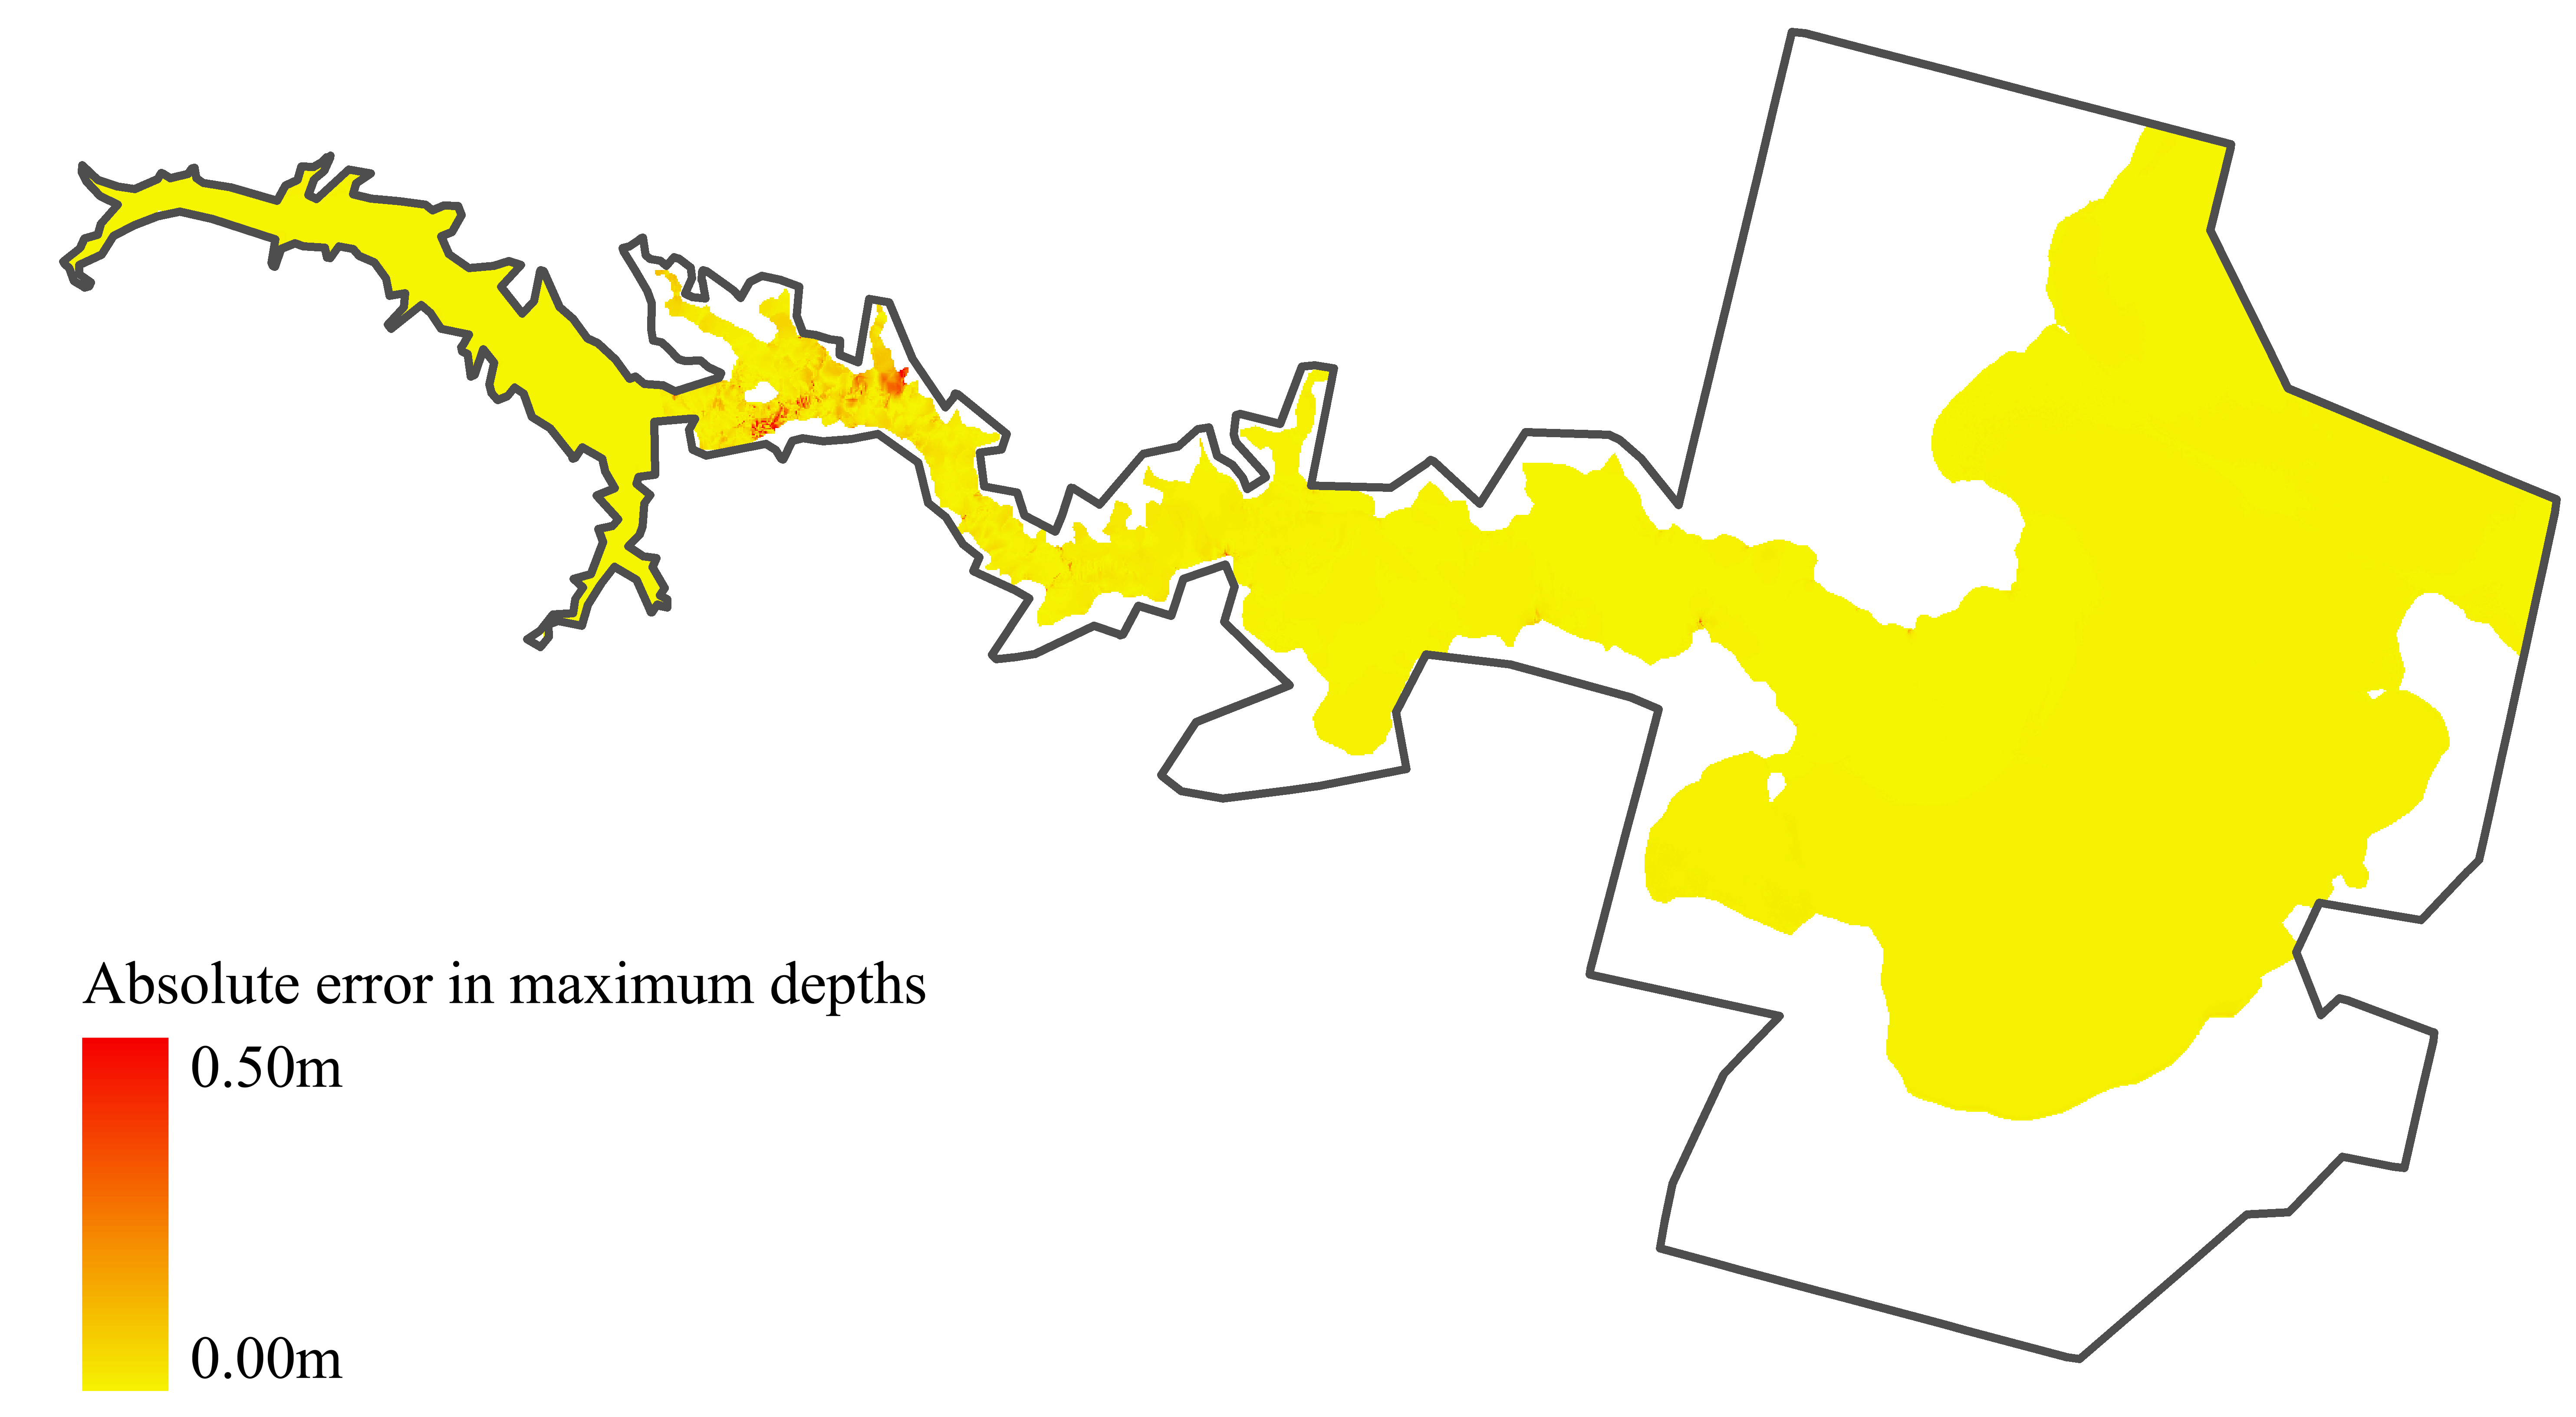
\includegraphics[width=1.0\textwidth]{heterogeneous-dev-figures/Figure_12_Colour.jpg}
	\caption{Spatial distribution of absolute errors in Malpasset, introduced in the maximum depths by using 32-bit floating-point after the Malpasset collapse, when compared to 64-bit results.}
	\label{FPErrorMax}
\end{figure*}

In all simulations carried out 32-bit computation was faster than 64-bit. There are substantial and significant differences in the results obtained however, which demonstrate that 32-bit introduces unacceptably large errors. The spatial distribution of errors in the final and maximum simulated depths are shown in Figure \ref{FPErrorFinal} and Figure \ref{FPErrorMax} respectively.  Errors in maximum depth are concentrated in areas with the greatest flow velocities and where shocks are observed immediately downstream of the dam, whereas the final depth errors mainly lie in the shoal zones of the catchment where water should drain. While the mean error in final depths with 32-bit is \(<0.05\)m, the greatest error was \(+1.89\)m, and for the maximum depths the greatest error was \(+0.85\)m. The technique adopted herein uses free-surface level as a conserved variable instead of depth, which reduces the numerical resolution of shallow depths in particular. Whilst the localised errors may be a by-product of the specific numerical scheme employed herein, the author urges caution and encourages further research before 64-bit precision is dispensed with for performance over accuracy.

Other authors have previously reported the differences between 32- and 64-bit floating-point in terms of a mass balance error introduced by successive rounding \citep[e.g.][]{Brodtkorb2010a}, which potentially overlooks the significant magnitude of localised errors. Unlike this study they conclude that 32-bit floating-point provides an acceptable degree of accuracy. This difference stems from the different numerical scheme employed herein. Mixing different levels of precision remains a possibility. 

\section{Conclusions}

In this chapter, the numerical and computational performance of the software was tested using different processing devices and levels of floating-point precision. The numerical performance appears consistent with other software and published results, whilst the numerical scheme employed is shown to influence results significantly in some cases, suggesting second-order accuracy is important especially in dam-break scenarios or those with frequently-changing wet-and-dry fronts. 

In respect of the tests considered in this chapter, it can be determined that:

\begin{itemize}
	\item the numerical schemes employed are both capable of representing the well-balanced property, exhibiting a static condition over a complex and varying bed topography, without problem;
	\item there are limitations to the applicability of the first-order solution, when dealing with continually changing wet-dry fronts over a long time period with a high grid resolution, and thus for tidal applications (which have much in common with the dam-break over an emerging bed), a second-order solution may be required, whilst for most progressive flood cases (fluvial and pluvial) the zone of inundation generally only expands;
	\item even when a second-order solution is employed, the speed of the wave front may be underestimated for dam break situations, caused by a combination of the limitations and assumptions of the shallow water equations, and the numerical scheme's approach to maintaining stability;
	\item with adequate spatial discretisation, complex phenomena such as the interaction between shock and rarefaction waves can be simulated correctly, as evidenced by the dam-break against a fixed obstacle, but accepting there are nonetheless discrepancies when compared against laboratory measurements;
	\item flows of a very shallow depth can be correctly simulated, such as in the case of intense rainfall during the Glasgow benchmark case, where the results are consistent with commercial software;
	\item use of single-precision (32-bit) arithmetic introduced considerable errors in the mass conservation for Glasgow, and depths at a critical point for Malpasset, and hence cannot be recommended for general use, without thorough sensitivity testing;
	\item performance tuning parameters and options, such as caching interim values during a second-order simulation, and alignment of variables in memory, made very little difference to the overall computational performance in many cases;
	\item satisfactory results were achieved for tests in which flooding was caused by pluvial, dam failure, and defence failure mechanisms;
	\item the processing device used made no discernible difference in the results (typically fractions of a millimetre in depth); and
	\item whether the additional computational overhead associated with the second-order solution is worthwhile in real-world cases requires professional judgement, with respect to the other uncertainty inherent in topographic and observational data.
\end{itemize}

Clear performance benefits are evident from GPU computation when compared to multi-core CPU use, however most of the the simulations presented herein have not been sufficiently large to fully capitalise on the GPU benefits. Later chapters include simulations for entire cities, and present an opportunity to further explore the performance benefits in practical applications.
